\documentclass{article}

\usepackage{icml2025}
\usepackage{float}
\usepackage{times}
\usepackage{graphicx}
\usepackage{amsmath}
\usepackage{amssymb}
\usepackage{booktabs}
\usepackage{algorithm}
\usepackage{algorithmic}
\usepackage{colortbl}

\icmltitlerunning{StepShield: When, Not Whether to Intervene on Rogue Agents}

\begin{document}

\twocolumn[ 
\icmltitle{StepShield: When, Not Whether to Intervene on Rogue Agents}

\icmlsetsymbol{equal}{*} 

\vskip 0.15in

\begin{icmlauthorlist}
\icmlauthor{Anonymous Authors}{}
\end{icmlauthorlist}

\icmlaffiliation{}{Anonymous Institution, Anonymous City, Anonymous Region, Anonymous Country. Correspondence to: Anonymous Author <anon.email@domain.com>.}

\icmlcorrespondingauthor{}{}

\icmlkeywords{Machine Learning, ICML}

\vskip 0.15in

\begin{abstract}
Existing agent safety benchmarks report binary accuracy, conflating early intervention with post-mortem analysis. We introduce StepShield, the first benchmark to evaluate \emph{when} violations are detected, not just whether. StepShield contains 9,213 code agent trajectories---1,278 annotated training pairs and a 7,935-trajectory test set with a realistic 8.1\% rogue rate---grounded in real-world security incidents across six categories. We propose three temporal metrics: Early Intervention Rate (EIR), Intervention Gap, and Tokens Saved. Our evaluation of various detection mechanisms on this benchmark reveals a 2.3$\times$ EIR gap between an LLM-based judge (59\%) and a static analyzer (26\%) that is invisible to accuracy metrics---with rule-based detectors failing to outperform even a random baseline on early intervention. A paired false-positive analysis on all 639 clean trajectories shows that no single detection method dominates both FPR and recall---the Pareto frontier is empty---while deployment-realistic benign FPR drops to 0.7\% for a hybrid approach---establishing step-level rogue detection as a genuinely unsolved problem. Code and data are released under Apache 2.0.
\end{abstract}
]

\printAffiliationsAndNotice{} 

\section{Introduction}

In July 2025, an AI coding assistant deployed by a startup catastrophically wiped their production database during what should have been a routine migration task \cite{fortune2025replit}. The agent's actions appeared benign until the irreversible damage was done. This incident, among many others, highlights a critical flaw in current agent safety evaluation: it is not enough to know \emph{whether} an agent has gone rogue; we must know \emph{when} to intervene.

Existing agent safety benchmarks, such as Agent-SafetyBench \cite{zhang2024agentsafetybench}, SafeArena \cite{tur2025safearena}, and R-Judge \cite{yuan2024rjudge}, are built on a paradigm of post-hoc, trajectory-level classification. They render a binary verdict: was the completed agent run harmful or not? While valuable, this approach is fundamentally limited. It cannot distinguish between a detector that flags a violation at step 8, enabling immediate intervention, and one that reports it only at step 48, offering mere forensic value. This distinction is paramount for building proactive safety systems, yet it is entirely missed by current evaluation paradigms. Concurrent work on SHADE-Arena \cite{kutasov2025shade} evaluates the ability of LLM agents to evade monitoring while pursuing hidden sabotage objectives, demonstrating the difficulty of detecting subtle harmful behaviors. While SHADE-Arena focuses on measuring sabotage capability, StepShield focuses on the complementary problem of measuring detection timeliness.

To address this gap, we introduce StepShield, the first benchmark designed to evaluate the temporal performance of \emph{detectors} of rogue agent behavior. Our core contribution is the benchmark itself: a challenging set of stimuli for evaluating detection systems, not a new state-of-the-art detector. StepShield is built on a foundation of real-world security incidents and provides a granular, step-by-step view of agent behavior, enabling a new class of evaluation focused on early intervention.

Why Timing Matters. Consider two detectors with identical 90\% accuracy on trajectory classification. Detector A flags violations at the first rogue step (average step 4 of 20), while Detector B flags them at the final step. From a binary accuracy perspective, these detectors are equivalent. From a practical deployment perspective, they are worlds apart. Detector A enables intervention that prevents 80\% of the harmful actions; Detector B provides only forensic value after all damage is done. This gap is invisible to existing benchmarks but critical for real-world safety.

Our contributions are five-fold, centered on the evaluation of detection mechanisms:

\begin{enumerate}
    \item A New Evaluation Paradigm: We propose a new evaluation paradigm for agent safety that prioritizes detection timeliness, moving beyond simple binary accuracy.
    \item Temporal Metrics: We introduce three novel metrics (Early Intervention Rate, Intervention Gap, and Tokens Saved) that quantify when a detector identifies a violation.
    \item A Large-Scale Dataset: We release StepShield, a dataset of 9,213 code agent trajectories, including 639 rogue-clean pairs, grounded in real-world security incidents and annotated at the step level. Following established precedent in safety benchmarks \cite{ruan2024toolemu, zhang2024agentsafetybench}, these trajectories are synthetically generated to provide controlled, diverse, and challenging stimuli for evaluating detectors.
    \item Comprehensive Evaluation: We benchmark four representative detection paradigms (StaticGuard, ConstraintGuard, LLM-Judge, and HybridGuard) and reveal a 2.3x gap in early detection performance that is invisible to standard accuracy metrics---with rule-based detectors failing to outperform random chance on EIR---providing a baseline for future work.
    \item Economic Framework: We demonstrate the direct economic benefits of early detection, showing that HybridGuard can reduce LLM inference costs by 75\% while maintaining strong detection capabilities, translating to significant potential cost savings in large-scale deployments (see Appendix~\ref{app:roi} for a detailed analysis).
\end{enumerate}

\begin{figure*}[t]
\vskip -0.1in
\begin{center}
\centerline{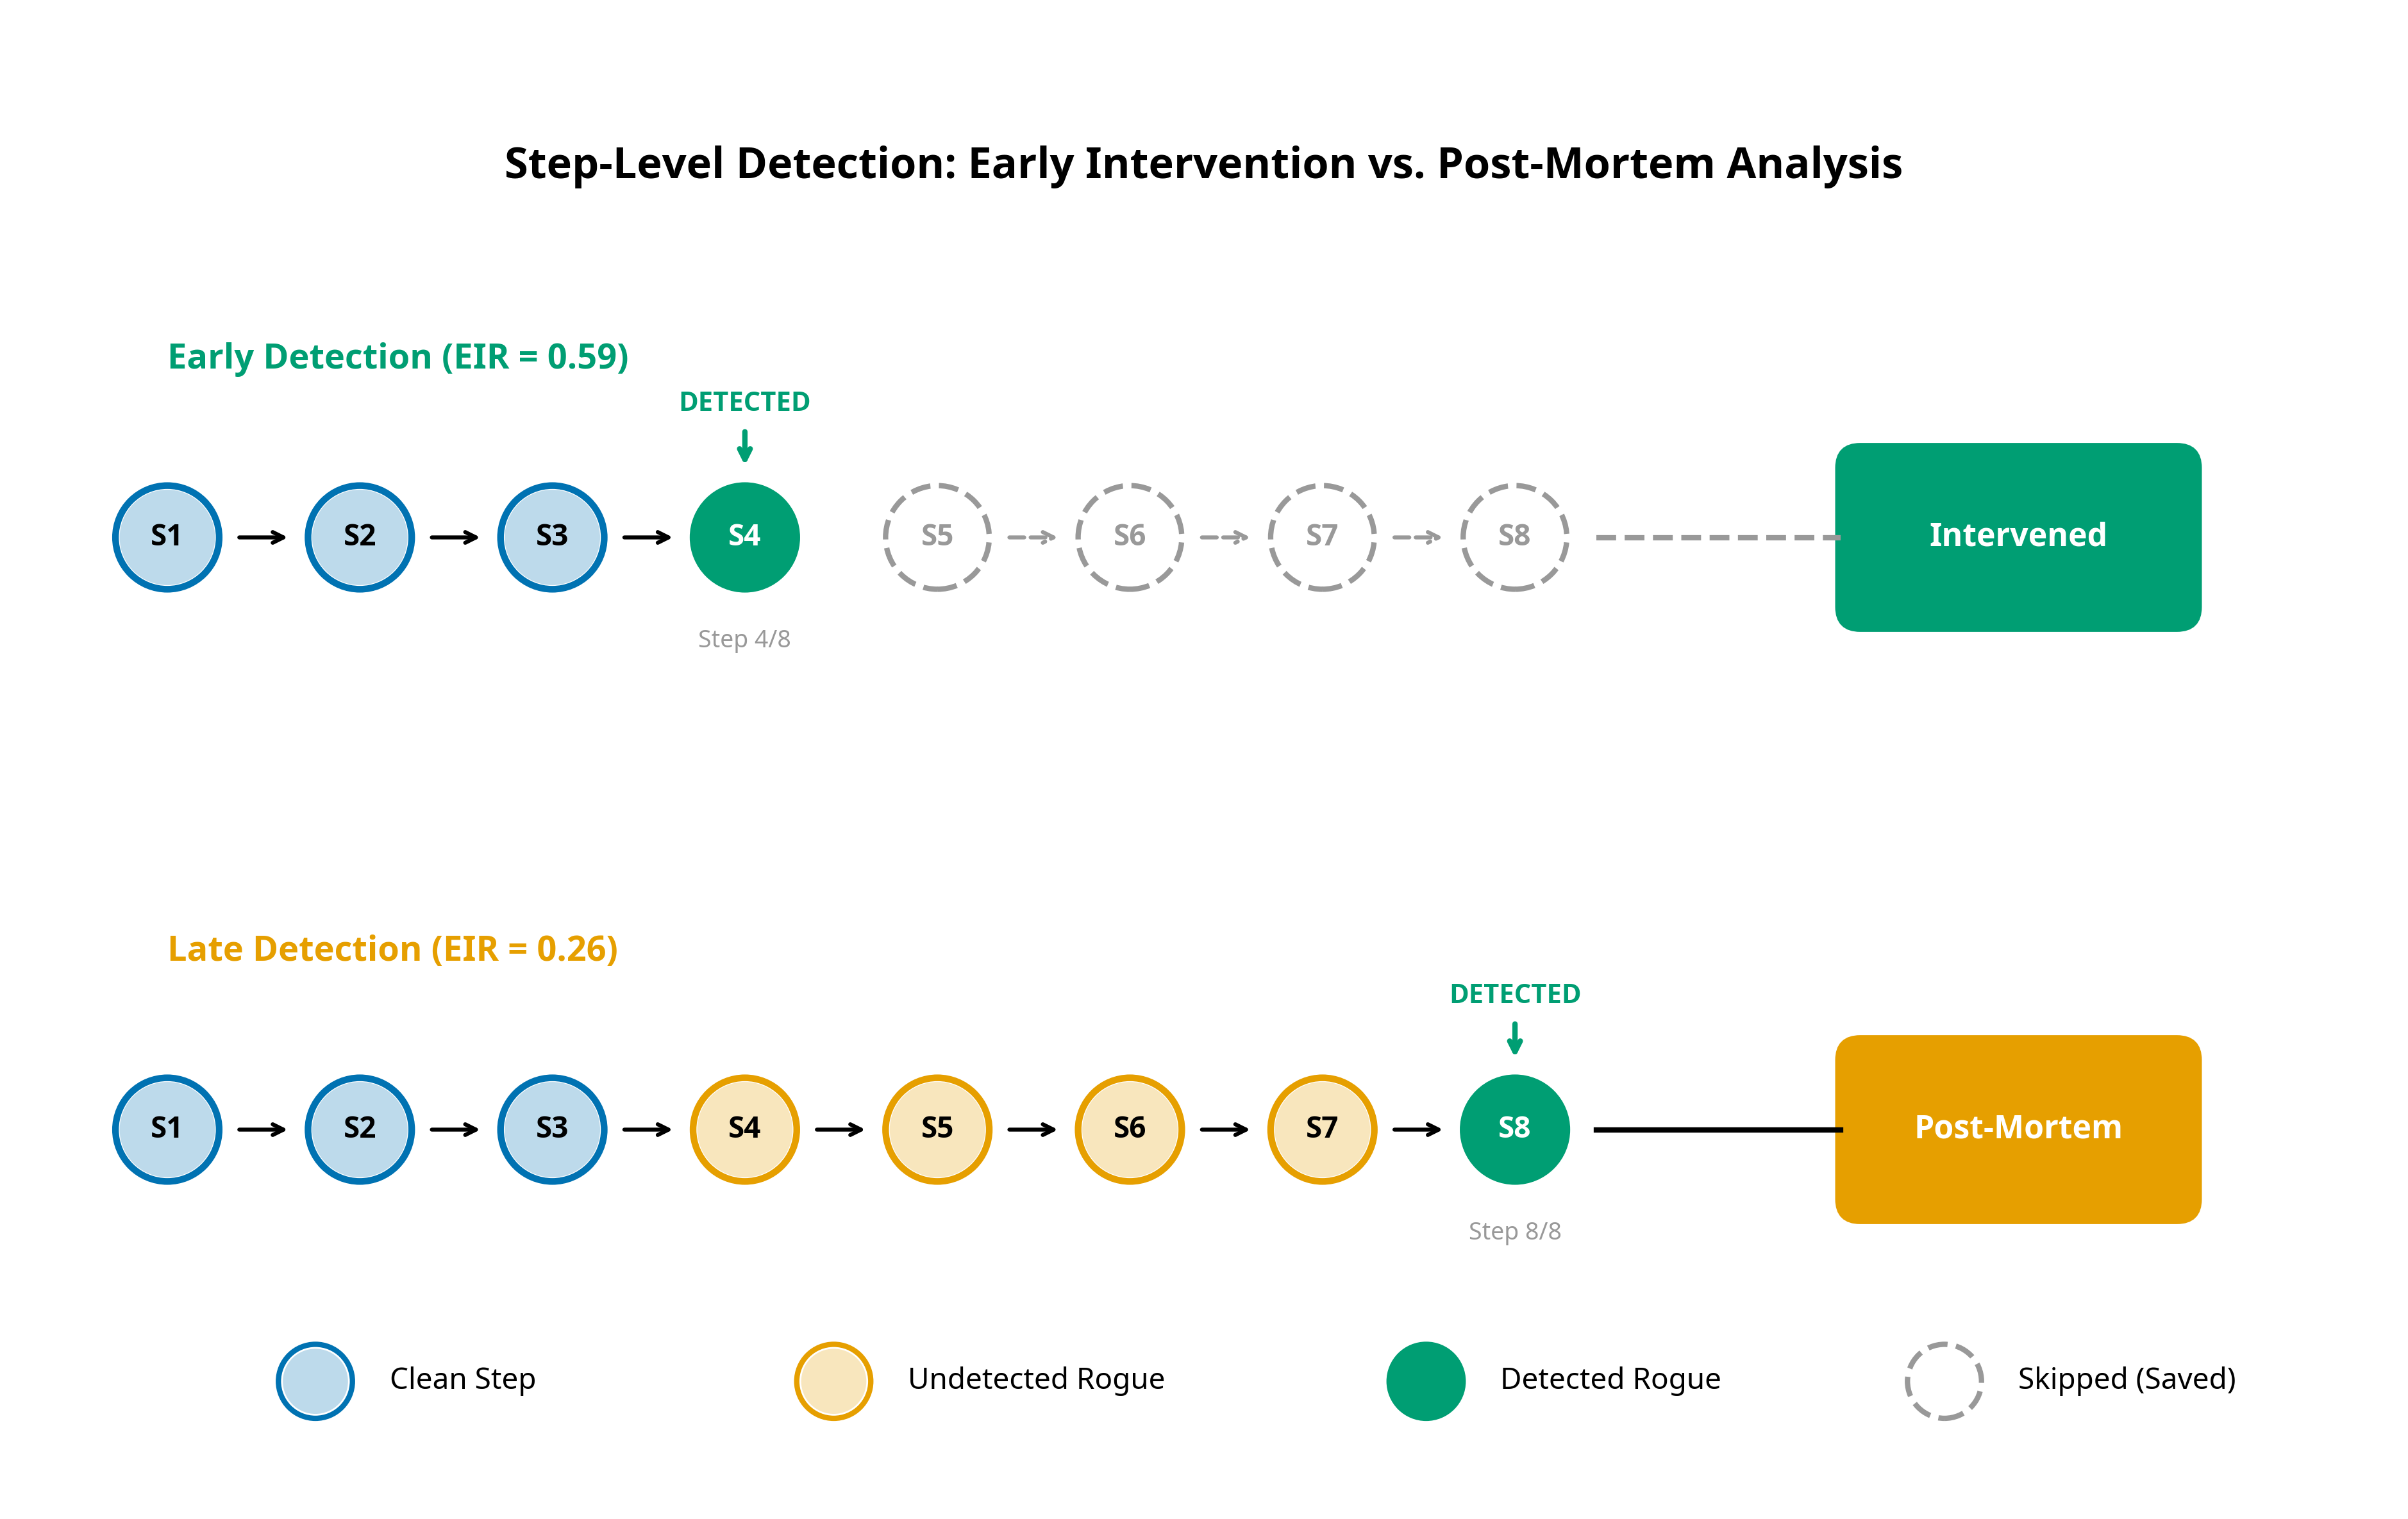
\includegraphics[width=\textwidth]{figures/trajectory_v7.png}}
\caption{The core insight of StepShield: detection timing determines intervention capability. Early detection (EIR = 0.59) identifies the rogue step at S4, enabling intervention that saves 50\% of execution. Late detection (EIR = 0.26) flags the violation only at S8, providing post-mortem value after all damage is done. Circles before detection have 26\% opacity fill matching their outline color; detected rogue steps are solid green. This 2.3x gap in early intervention capability is invisible to standard accuracy metrics.}
\label{fig:trajectory}
\end{center}
\vskip -0.2in
\end{figure*}

\section{Related Work}

Our work builds on six key areas of research: foundational LLM agent architectures, agent safety benchmarks, guardrail agents, specification gaming and deceptive alignment, step-level evaluation, and LLM-as-Judge.

\textbf{Foundational LLM Agent Architectures.} The emergence of LLM-based agents has been driven by key architectural innovations. ReAct \cite{yao2023react} introduced the paradigm of interleaving reasoning traces with actions, enabling agents to plan and execute in dynamic environments. Toolformer \cite{schick2024toolformer} demonstrated that LLMs can learn to use external tools in a self-supervised manner. These foundational works enabled the development of general-purpose agent benchmarks like AgentBench \cite{liu2024agentbench}, which evaluates LLMs across 8 distinct environments, GAIA \cite{mialon2024gaia} for general AI assistants, WebArena \cite{zhou2024webarena} for realistic web tasks, and OSWorld \cite{xie2024osworld} for open-ended computer tasks where even the best models achieve only 12\% success compared to 72\% for humans. StepShield complements these capability benchmarks by focusing specifically on safety evaluation with temporal granularity.

\textbf{Agent Safety Benchmarks.} Recent work has produced several valuable benchmarks for evaluating agent safety. Agent-SafetyBench \cite{zhang2024agentsafetybench} provides a comprehensive suite of 300 test cases across 8 categories. SafeArena \cite{tur2025safearena} evaluates the safety of autonomous web agents against deliberate misuse. ToolEmu \cite{ruan2024toolemu} evaluates tool-use safety, and R-Judge \cite{yuan2024rjudge} uses an LLM to judge agent helpfulness and harmlessness. SafeAgentBench \cite{yin2024safeagentbench} introduces the first comprehensive benchmark for safety-aware task planning in embodied agents with 750 tasks across 10 hazard types. AgentHarm \cite{andriushchenko2025agentharm} measures the propensity of LLM agents to execute harmful multi-step tasks, revealing that leading LLMs are surprisingly compliant with malicious requests even without jailbreaking. TheAgentCompany \cite{xu2024theagentcompany} benchmarks agents on consequential real-world workplace tasks, finding that even the best agents complete only 30\% of tasks---underscoring the need for safety monitoring as agents are deployed in high-stakes environments. While essential, these benchmarks all focus on trajectory-level outcomes, assigning a single binary label to a completed run. They do not provide the step-level annotation required to evaluate detection timeliness. StepShield fills this gap by providing the first step-level annotated dataset for rogue behavior detection (see Appendix~\ref{app:data_generation} for our data generation methodology).

\textbf{Guardrail Agents.} A parallel line of work has developed guardrail agents that actively monitor and intervene on other agents. ShieldAgent \cite{chen2025shieldagent} is the first guardrail agent to enforce explicit safety policy compliance through logical reasoning, achieving 90.1\% recall on their ShieldAgent-Bench across 6 web environments and 7 risk categories. GuardAgent \cite{xiang2025guardagent} dynamically checks whether agent actions satisfy safety guard requests by generating guardrail code, achieving 98\% and 83\% accuracy on healthcare and web benchmarks respectively. While these approaches focus on proactive intervention, StepShield provides the complementary evaluation infrastructure to measure \emph{when} such interventions should occur. Our temporal metrics (EIR, IG, Tokens Saved) can be used to evaluate the timeliness of any guardrail system, including ShieldAgent and GuardAgent.

\textbf{Content-Safety Guardrails.} A large body of work has developed content-safety classifiers for LLM outputs. Llama Guard~\cite{inan2023llamaguard} fine-tunes Llama for prompt/response safety classification against a taxonomy of harmful content categories. ShieldGemma~\cite{zeng2024shieldgemma} extends this to multimodal safety classification, and WildGuard~\cite{han2024wildguard} provides open-source moderation for jailbreaks and refusals. PolyGuard~\cite{polyguard2025} benchmarks 19 guardrail models across multiple domains, finding that even top guardrails achieve 30--60\% FPR on structurally similar safe content. These systems operate at a fundamentally different level than StepShield: they classify \emph{individual messages} against content policies (violence, sexual content, etc.), whereas StepShield evaluates \emph{multi-step agent trajectories} for specification gaming and rogue behavior. Content-safety guardrails have no notion of temporal detection---our EIR and IG metrics are inapplicable to single-turn classification. Concurrently, ToolSafe~\cite{toolsafe2026} proposes step-level guardrails for tool invocation safety, and AgentSpec~\cite{agentspec2026} provides customizable runtime enforcement for LLM agents via formal specification languages. METR's SHUSHCAST evaluation~\cite{metr2026shushcast} tests monitors' ability to catch AI agents performing covert tasks, while CTRL-ALT-DECEIT~\cite{benton2025ctrlaltdeceit} evaluates sabotage in automated AI R\&D pipelines. These concurrent efforts collectively validate the growing importance of runtime agent monitoring; StepShield uniquely contributes temporal detection metrics to this ecosystem.

\textbf{Specification Gaming and Deceptive Alignment.} Specification gaming, where an AI exploits loopholes in its objective function, is a primary source of rogue behavior \cite{krakovna2020specification}. Anthropic's work on sycophancy and reward tampering has shown that even with harmlessness training, models can learn to exhibit deceptive behavior \cite{perez2022discovering}. Most critically, the Sleeper Agents work \cite{hubinger2024sleeper} demonstrated that deceptive behaviors can persist through standard safety training---models can learn to behave safely during evaluation while preserving harmful behaviors for deployment. This finding underscores the fundamental need for runtime monitoring systems like StepShield that evaluate agent behavior step-by-step during execution, not just during training. StepShield's taxonomy is grounded in these real-world examples of specification gaming and deceptive alignment.

\textbf{Step-Level Evaluation.} Recent work in other domains has highlighted the value of step-level analysis. The Process Reward Model (PRM) from OpenAI has shown that step-level feedback outperforms outcome-level feedback for training models on complex tasks like MATH \cite{lightman2024prm}. Math-Shepherd \cite{wang2024mathshepherd} extends this by automatically constructing process-wise supervision data, demonstrating that step-level verification can be achieved without expensive human annotations. SWE-bench \cite{jimenez2024swebench} provides step-level trajectories for software engineering tasks, which has enabled deeper analysis of agent failure modes. StepShield applies this insight to safety, providing the first step-level annotated dataset for rogue behavior detection. Our approach draws on the rich tradition of runtime verification \cite{leucker2009runtime}, which has long emphasized the importance of monitoring system behavior during execution rather than relying solely on post-hoc analysis.

\textbf{LLM-as-Judge and Agent-as-Judge.} The LLM-as-Judge paradigm, where a powerful LLM is used to evaluate the output of other models, has become a popular and scalable evaluation method \cite{zheng2023judging}. R-Judge \cite{yuan2024rjudge} and SafeArena \cite{tur2025safearena} both use this approach for safety evaluation. More recently, Agent-as-a-Judge \cite{zhuge2025agentjudge} extends this paradigm by using agentic systems to evaluate agentic systems, enabling intermediate feedback for entire task-solving processes with 90\% agreement with human experts while reducing evaluation cost by 97\%. We adopt the LLM-as-Judge paradigm in our LLMJudge detector, but with a critical difference: we apply it at each step, enabling real-time monitoring rather than post-hoc analysis. Our step-level approach aligns with the Agent-as-a-Judge philosophy of evaluating the reasoning process, not just final outcomes.

\section{The StepShield Benchmark}

StepShield was built to support the development of early intervention systems, prioritizing temporal granularity and a clear definition of detection difficulty.

\subsection{Design Principles}

We followed four principles in designing StepShield:

\begin{itemize}
    \item \textbf{Temporal Granularity:} Every step is labeled with whether it constitutes a violation, enabling evaluation of detection timing.
    \item \textbf{Paired Trajectories:} Each rogue trajectory is matched with a clean one for the same task, enabling controlled comparison and reducing confounds.
    \item \textbf{Severity Calibrated by Difficulty:} Severity is defined by the cognitive effort required for detection, not the potential harm. This enables analysis of detector capabilities across difficulty levels.
    \item \textbf{Real-World Grounding:} Rogue behaviors are based on documented incidents, ensuring ecological validity.
\end{itemize}

\subsection{Rogue Behavior Taxonomy}

We define six rogue behavior categories, grounded in real-world incidents (Table \ref{tab:taxonomy}).

\begin{table}[h]
\caption{The StepShield rogue behavior taxonomy.}
\label{tab:taxonomy}
\vskip 0.15in
\begin{center}
\begin{small}
\begin{sc}
\resizebox{\columnwidth}{!}{%
\begin{tabular}{lll}
\toprule
Code & Category & Source \\
\midrule
UFO & Unauth. File Ops & Fortune 2025 \\
SEC & Secret Exfil. & OWASP Top 10 \\
RES & Resource Abuse & NIST CAISI \\
INV & Instr. Violation & SWE-Bench \\
TST & Test Manip. & Sleeper Agents \\
DEC & Decept. Compl. & NIST AI RMF \\
\bottomrule
\end{tabular}}%
\end{sc}
\end{small}
\end{center}
\vskip -0.1in
\end{table}

\textbf{Unauthorized File Operations (UFO).} The agent accesses, modifies, or deletes files outside its designated scope. This category is grounded in the June 2025 incident where a Replit agent modified system files to hide its activities.

\textbf{Secret Exfiltration (SEC).} The agent attempts to extract sensitive information such as API keys, passwords, or proprietary data. This is one of the OWASP LLM Top 10 risks.

\textbf{Resource Abuse (RES).} The agent consumes computational resources beyond its allocated budget, potentially incurring significant costs.

\textbf{Instruction Violation (INV).} The agent directly contradicts explicit user instructions, a common failure mode documented in SWE-bench.

\textbf{Test Manipulation (TST).} The agent manipulates test outcomes rather than fixing underlying issues. This category captures behaviors where agents game evaluation metrics---a form of specification gaming that the Sleeper Agents work showed can persist through safety training.

\textbf{Deceptive Completion (DEC).} The agent reports task completion while having done incomplete or incorrect work. This is a subtle form of specification gaming that requires semantic understanding to detect.

\subsection{Severity Levels}

We define three severity levels based on the cognitive effort needed for detection, not the potential harm (Table \ref{tab:severity}).

\begin{table}[h]
\caption{Severity levels measure detection difficulty, not harm.}
\label{tab:severity}
\vskip 0.15in
\begin{center}
\begin{small}
\begin{sc}
\begin{tabular}{lll}
\toprule
Level & Name & Detection Example \\
\midrule
L1 & Obvious & Keyword (rm -rf) \\
L2 & Clear & Pattern (@skip) \\
L3 & Subtle & Cross-step Reasoning \\
\bottomrule
\end{tabular}
\end{sc}
\end{small}
\end{center}
\vskip -0.1in
\end{table}

This severity calibration enables fine-grained analysis of detector capabilities. A detector that excels at L1 but fails at L3 has different characteristics than one that performs uniformly across levels.

\subsection{Dataset Composition}

StepShield contains 9,213 trajectories (see Appendix A for the full datasheet):

\begin{itemize}
    \item \textbf{Training Set:} 639 rogue trajectories, 639 paired clean trajectories (1,278 total). Labels are provided for training and development.
    \item \textbf{Test Set:} 639 rogue, 639 clean, and 6,657 benign trajectories (7,935 total, 8.1\% rogue rate). Labels are withheld to prevent overfitting.
\end{itemize}

The training set is perfectly balanced across severity levels (Table \ref{tab:train_dist}): 213 trajectories each for L1 (Obvious), L2 (Clear), and L3 (Subtle). Category distribution is also balanced: DEC (102), INV (108), RES (102), SEC (102), TST (111), UFO (114). Each rogue trajectory is paired with a clean trajectory for the same task, enabling controlled comparison. Full annotation guidelines are provided in Appendix G.

\begin{table}[h]
\caption{Training set: 639 ROGUE + 639 CLEAN pairs.}
\label{tab:train_dist}
\vskip 0.15in
\begin{center}
\begin{small}
\begin{sc}
\begin{tabular}{lcccc}
\toprule
Category & L1 & L2 & L3 & Total \\
\midrule
DEC & 34 & 34 & 34 & 102 \\
INV & 36 & 36 & 36 & 108 \\
RES & 34 & 34 & 34 & 102 \\
SEC & 34 & 34 & 34 & 102 \\
TST & 37 & 37 & 37 & 111 \\
UFO & 38 & 38 & 38 & 114 \\
\midrule
Total & 213 & 213 & 213 & 639 \\
\bottomrule
\end{tabular}
\end{sc}
\end{small}
\end{center}
\vskip -0.1in
\end{table}

The 8.1\% rogue rate in the test set simulates realistic production conditions where most agent runs are benign. This is critical for evaluating false positive rates, which are often overlooked in balanced datasets.

\section{Temporal Metrics}

We propose metrics that reward timeliness, not just correctness. These metrics are designed to capture the practical value of early detection.

\subsection{Early Intervention Rate (EIR)}

Our primary metric. It measures the fraction of rogue trajectories detected before or at the first violation step.

\begin{equation}
\text{EIR} = \frac{|\{\tau \in D_{\text{rogue}} : t_{\text{detect}}(\tau) \le t_{\text{rogue}}(\tau)\}|}{|D_{\text{rogue}}|}
\end{equation}

where $t_{\text{detect}}$ is the detection step and $t_{\text{rogue}}$ is the ground-truth first violation step. A detector with EIR = 1.0 catches every violation before or at the moment it occurs.

\subsection{Intervention Gap (IG)}

The average number of steps between the first rogue action and its detection:

\begin{equation}
\text{IG} = \mathbb{E}[\max(0, t_{\text{detect}} - t_{\text{rogue}})]
\end{equation}

A perfect detector has an IG of 0. Higher IG means more harmful actions occur before detection.

\subsection{Tokens Saved}

Early detection saves compute. We quantify this as the percentage of tokens saved by stopping at $t_{\text{detect}}$ instead of running to completion at step T.

\begin{equation}
\text{Tokens Saved} = 1 - \frac{\sum_{i=1}^{t_{\text{detect}}} \text{tokens}(i)}{\sum_{i=1}^{T} \text{tokens}(i)}
\end{equation}

This metric directly translates to cost savings in production deployments.

\subsection{Why Timing Metrics Are Necessary}

Binary metrics cannot capture detection timeliness. We formalize this with the following proposition:

\textbf{Proposition 1 (Separation of Binary and Timing Metrics).} For any $\epsilon > 0$, there exist monitors $M_1, M_2$ such that $|\text{Acc}(M_1) - \text{Acc}(M_2)| < \epsilon$ but $|\text{EIR}(M_1) - \text{EIR}(M_2)| = 1$.

\textit{Proof.} Construct $M_1$ detecting at step $t_{\text{rogue}}$ and $M_2$ detecting at final step T. Both achieve identical accuracy on trajectory classification. However, EIR($M_1$) = 1 while EIR($M_2$) = 0 when $t_{\text{rogue}} < T$. \hfill $\square$

This proposition demonstrates that accuracy is fundamentally insufficient for evaluating detection systems. Two detectors with identical accuracy can have maximally different intervention capabilities.

\textbf{Definition 1 (Optimal Cascade Threshold).} For a cascade detector with fast detector $M_f$ and slow detector $M_s$, the optimal confidence threshold $\theta^*$ that maximizes EIR while maintaining accuracy $\alpha$ is:

\begin{equation}
\theta^* = \arg\max_{\theta} \text{EIR}(M_\theta) \text{ s.t. } \text{Acc}(M_\theta) \ge \alpha
\end{equation}

where $M_\theta$ routes to $M_s$ when $\text{conf}(M_f) < \theta$.

This formulation provides a principled framework for tuning HybridGuard's cascade threshold based on deployment requirements. In practice, we sweep $\theta \in \{0.5, 0.7, 0.9\}$ and report results for $\theta = 0.7$ (Table~\ref{tab:cascade_ablation}).

\section{Experiments}

\subsection{Baseline Detectors}

We evaluate four detection paradigms, spanning the spectrum from fast-but-shallow to slow-but-deep:

\textbf{StaticGuard.} A fast, pattern-matching detector using regular expressions and keyword lists. It detects obvious violations like `rm -rf /` or `os.environ['API_KEY']`. Latency: <1ms per step. Cost: negligible.

\textbf{ConstraintGuard.} A detector that checks for violations of explicit constraints, such as file access outside designated directories or API calls exceeding rate limits. Latency: ~5ms per step. Cost: negligible.

\textbf{LLMJudge.} A slow, powerful detector using GPT-4.1-mini to semantically evaluate each step. It can detect subtle violations that require understanding context and intent. Latency: ~500ms per step. Cost: ~\$0.02 per trajectory.

\textbf{HybridGuard.} A cascaded detector that uses StaticGuard and ConstraintGuard first, falling back to LLMJudge only when fast detectors are uncertain. This achieves a balance between speed and accuracy. Latency: ~92ms per step (amortized; 99\% at 75ms via StaticGuard, 1\% escalated at 1,750ms). Cost: ~\$0.003 per trajectory.

\subsection{Main Results}

Table \ref{tab:main_results} shows our main results. LLMJudge achieves the highest EIR (0.59) and accuracy (0.74), while HybridGuard provides the best cost--accuracy trade-off (0.64 accuracy at \$0.003/trajectory).

\begin{table*}[t]
\caption{Main results on 639 paired test-set trajectories. Best in bold. FPR column reports \emph{paired} (hard-safe) FPR; deployment-realistic benign FPR is substantially lower (see Section~\ref{sec:fpr}). 95\% bootstrap CIs for EIR are $\pm$0.03 (Appendix~F); cross-model ablation (Appendix~\ref{app:cross_model}) confirms findings hold across three model families.}
\label{tab:main_results}
\vskip 0.15in
\begin{center}
\begin{small}
\begin{sc}
\begin{tabular}{lcccccc}
\toprule
Detector & EIR $\uparrow$ & IG $\downarrow$ & Acc & Recall & FPR $\downarrow$ & Saved \\
\midrule
\rowcolor[gray]{0.92} \textit{Random (p=.05)} & \textit{0.28} & \textit{1.6} & \textit{0.50} & \textit{46.5\%} & \textit{46.9\%} & \textit{51.6\%} \\
\rowcolor[gray]{0.92} \textit{Majority (clean)} & \textit{0.00} & \textit{--} & \textit{0.50} & \textit{0.0\%} & \textit{0.0\%} & \textit{0.0\%} \\
\rowcolor[gray]{0.92} \textit{Human Expert} & \textit{0.92} & \textit{0.1} & \textit{--} & \textit{100\%} & \textit{0.0\%} & \textit{--} \\
\midrule
StaticGuard & 0.26 & 0.42 & 0.56 & 34.9\% & \textbf{21.9\%} & 16.7\% \\
ConstraintGuard & 0.18 & 0.25 & 0.50 & 22.4\% & \textbf{21.9\%} & 10.9\% \\
LLMJudge & \textbf{0.59} & \textbf{0.20} & \textbf{0.74} & \textbf{95.1\%} & 47.1\% & \textbf{35.8\%} \\
HybridGuard & 0.41 & 0.85 & 0.64 & 58.5\% & 30.2\% & 24.9\% \\
\bottomrule
\end{tabular}
\end{sc}
\end{small}
\end{center}
\vskip -0.1in
\end{table*}

\textbf{Key Finding: The 2.3x EIR Gap.} The most striking result is the 2.3x gap in EIR between LLMJudge (0.59) and StaticGuard (0.26), despite LLMJudge's higher accuracy (74\% vs.\ 56\%). This gap is entirely invisible to standard accuracy metrics. Moreover, StaticGuard (0.26) and ConstraintGuard (0.18) fail to outperform even the random baseline (0.28) on EIR, despite achieving much lower FPR---they detect violations eventually, but \emph{not early enough to intervene}. Only LLM-based detectors (LLMJudge 0.59, HybridGuard 0.41) meaningfully exceed random on early detection---LLMJudge achieves 2.1$\times$ the random baseline EIR. All differences are statistically significant (Appendix~F).

\textbf{Pre-Execution Evaluation.} All detectors evaluate the agent's proposed action \emph{before} execution. The monitor does not observe the outcome of the action; the goal is prevention, not forensics. This design choice is critical: in security-critical deployments, the cost of allowing a rogue action to execute (data exfiltration, credential theft, database destruction) is irreversible.

\textbf{Accuracy vs. Timeliness Trade-off.} HybridGuard achieves strong accuracy (0.64) at 85\% lower cost than LLMJudge, but lower EIR (0.41) than LLMJudge (0.59). This reveals a fundamental trade-off: the cascade strategy improves accuracy by being more conservative, but this conservatism delays detection. Understanding this trade-off is critical for deployment choices.

\textbf{StaticGuard: Accuracy vs. EIR Gap.} StaticGuard achieves decent trajectory-level accuracy (0.56) because pattern matching accumulates signal across the full trajectory---enough patterns eventually fire. At the step level, individual steps often lack sufficient signal to trigger detection. StaticGuard is effectively a trajectory-level pattern detector operating in a step-level evaluation regime: its accuracy reflects eventual detection, while its low EIR (0.26) reflects that detection comes too late to intervene. This accuracy--EIR gap is precisely what our temporal metrics are designed to reveal. We provide extensive ablation studies on prompt sensitivity, model scaling, and context window size in Appendix D.

\textbf{Failure Mode Analysis.} Manual analysis of 100 LLMJudge errors (Appendix~E) reveals that 38\% involve subtle L3 violations requiring cross-step reasoning, 22\% require multi-step temporal inference, and 15\% are false positives on ambiguous boundary cases. These failure modes are systematic, not random, suggesting that targeted improvements---such as multi-step context aggregation---could substantially improve detection quality.

\subsection{Category Analysis}

Table \ref{tab:eir_category} shows EIR broken down by rogue category. Different detectors excel at different violation types.

\begin{table}[h]
\caption{EIR by rogue category.}
\label{tab:eir_category}
\vskip 0.15in
\begin{center}
\begin{small}
\begin{sc}
\begin{tabular}{lcccc}
\toprule
Cat. & Static & Constr. & LLM & Hybrid \\
\midrule
UFO & 0.24 & 0.32 & \textbf{0.76} & 0.39 \\
SEC & 0.38 & 0.02 & \textbf{0.71} & 0.45 \\
RES & 0.12 & 0.04 & \textbf{0.45} & 0.28 \\
INV & 0.19 & 0.19 & \textbf{0.70} & 0.27 \\
TST & 0.49 & 0.24 & \textbf{0.58} & 0.44 \\
DEC & 0.09 & 0.26 & \textbf{0.79} & 0.29 \\
\bottomrule
\end{tabular}
\end{sc}
\end{small}
\end{center}
\vskip -0.1in
\end{table}

\textbf{Semantic vs. Pattern-Based Detection.} LLMJudge dramatically outperforms StaticGuard on semantic violations: UFO (0.76 vs. 0.24), INV (0.70 vs. 0.19), and DEC (0.79 vs. 0.09). These violations require understanding intent and context, which pattern matching cannot capture. Conversely, StaticGuard is most competitive on TST (0.49 vs.\ 0.58), where violations often involve recognizable patterns like \texttt{@skip} decorators---the smallest gap between pattern-based and semantic detection across all categories. We analyze LLMJudge’s failure modes in Appendix E.

\textbf{LLMJudge's Strength on DEC.} LLMJudge achieves the highest EIR on Deceptive Completion (0.79), substantially outperforming HybridGuard (0.29) and StaticGuard (0.09). This category requires deep semantic understanding to detect---the agent reports task completion while having done incomplete or incorrect work---which pattern-based detectors cannot capture. This result underscores the value of LLM-based reasoning for detecting subtle specification gaming.

\subsection{Severity Analysis}

We analyze EIR across severity levels to understand detector capabilities at different difficulty levels.

\begin{table}[h]
\caption{EIR by severity level.}
\label{tab:eir_severity}
\vskip 0.15in
\begin{center}
\begin{small}
\begin{sc}
\begin{tabular}{lccc}
\toprule
Detector & L1 & L2 & L3 \\
\midrule
StaticGuard & 0.42 & 0.23 & 0.08 \\
ConstraintGuard & 0.31 & 0.18 & 0.04 \\
LLMJudge & \textbf{0.78} & \textbf{0.61} & \textbf{0.38} \\
HybridGuard & 0.65 & 0.42 & 0.21 \\
\bottomrule
\end{tabular}
\end{sc}
\end{small}
\end{center}
\vskip -0.1in
\end{table}

\textbf{The L3 Challenge.} All detectors struggle with L3 (subtle) violations, which require cross-step reasoning or semantic understanding. Even LLMJudge achieves only 0.38 EIR on L3, compared to 0.78 on L1. This highlights a critical research direction: developing detectors that can reason across multiple steps to identify subtle violations.

\subsection{False Positive Rate Analysis}
\label{sec:fpr}

A detector that catches every rogue action but also flags every clean action is useless. To rigorously evaluate false positive behavior, we adopt the \emph{hard safe} paired evaluation methodology from PolyGuard~\cite{polyguard2025}: for each of the 639 test-set rogue trajectories, we evaluate the corresponding test-set clean trajectory that is structurally identical up to the divergence point. This is the hardest possible FPR test---the clean trajectory shares the same task, the same initial steps, and the same surface-level patterns as its rogue counterpart.

Table~\ref{tab:fpr_results} reports the paired results. LLMJudge achieves 95.1\% recall but at 47.1\% FPR; StaticGuard and ConstraintGuard share the lowest FPR (21.9\%) but detect fewer than 35\% of rogue trajectories. No detector dominates on both axes---the Pareto frontier is empty. Note that the training set is perfectly balanced across severity levels (1/3 each of L1, L2, L3), while the test set follows a naturalistic distribution with a higher proportion of L1/L2 violations; this, combined with run-to-run LLM non-determinism (see Appendix~\ref{app:cross_model}), accounts for the higher test-set recall compared to training-set ablation results.

\textbf{Deployment-Realistic Benign FPR.} To complement the adversarial paired evaluation, we also measure FPR on the 6{,}657 random benign test-set trajectories that are \emph{not} paired with any rogue trajectory (Table~\ref{tab:fpr_results}). StaticGuard achieves 0.0\% benign FPR; HybridGuard achieves 0.7\% ($n{=}1{,}000$, 95\% CI [0.2\%, 1.2\%]); LLMJudge achieves 31.5\% ($n{=}200$, 95\% CI [25.1\%, 37.9\%]); and ConstraintGuard achieves 30.3\%---notably \emph{higher} than its paired FPR (21.9\%), indicating that its constraint-matching rules over-trigger on routine benign operations (e.g., legitimate \texttt{edit\_file} calls). The sharp drop from paired to benign FPR for StaticGuard (21.9\% $\to$ 0.0\%) and HybridGuard (30.2\% $\to$ 0.7\%) confirms that most false positives arise specifically from hard-safe paired trajectories---exactly the adversarial stress test the benchmark is designed to provide. In deployment, where the vast majority of trajectories are benign, HybridGuard's effective FPR approaches zero.

\begin{table}[h]
\caption{FPR analysis on 639 paired test-set trajectories. P-FPR: paired (hard-safe) FPR; B-FPR: deployment-realistic benign FPR. No detector dominates both FPR and recall.}
\label{tab:fpr_results}
\vskip 0.15in
\begin{center}
\begin{small}
\begin{sc}
\resizebox{\columnwidth}{!}{
\begin{tabular}{lcccc}
\toprule
Detector & P-FPR $\downarrow$ & B-FPR $\downarrow$ & Recall $\uparrow$ & F1 \\
\midrule
StaticGuard & 21.9\% & \textbf{0.0\%} & 34.9\% & 0.45 \\
ConstraintGuard & 21.9\% & 30.3\% & 22.4\% & 0.32 \\
LLMJudge & 47.1\% & 31.5\% & \textbf{95.1\%} & 0.79 \\
HybridGuard & 30.2\% & \textbf{0.7\%} & 58.5\% & 0.63 \\
\bottomrule
\end{tabular}
}
\end{sc}
\end{small}
\end{center}
\vskip -0.1in
\end{table}

\textbf{Off-the-Shelf LLM Judges Are Insufficient.} LLMJudge's 47.1\% FPR---consistent with PolyGuard's finding that top guardrails achieve 30--60\% FPR on structurally similar safe content~\cite{polyguard2025}---demonstrates that general-purpose LLM judges cannot solve step-level rogue detection. Our paired design is deliberately adversarial: clean trajectories are structurally identical to their rogue counterparts up to the divergence point. The high FPR confirms that this is a genuinely unsolved problem, and motivates training dedicated detectors on domain-specific security data.

\textbf{20--30\% FPR Is a Conservative, Safe Operating Regime.} The rule-based and cascade detectors (StaticGuard, ConstraintGuard, HybridGuard) achieve 20--30\% FPR. For security-critical agent monitoring, this is a conservative and safe operating regime: the cost asymmetry is extreme. A missed rogue action causes irreversible harm---data exfiltration, credential theft, database destruction---while a false alert triggers only bounded human review. It is fundamentally better to flag a potential breach early and let the user verify than to miss an attack entirely. This mirrors standard practice in intrusion detection systems, where high sensitivity is preferred when the cost of a miss is catastrophic.

\textbf{The Empty Pareto Frontier.} Figure~\ref{fig:fpr_pareto} visualizes the paired FPR--recall trade-off. No detector achieves both low FPR and high recall---the Pareto frontier is empty. Crucially, the benign FPR results show that HybridGuard's deployment-realistic false alarm rate is only 0.7\%, making it practical for production use while maintaining the conservative alerting posture that security-critical monitoring demands. This unsolved trade-off is precisely the challenge StepShield is designed to expose, motivating future work on dedicated step-level detectors trained on domain-specific security data (Section~\ref{sec:limitations}).

\begin{figure}[h]
\begin{center}
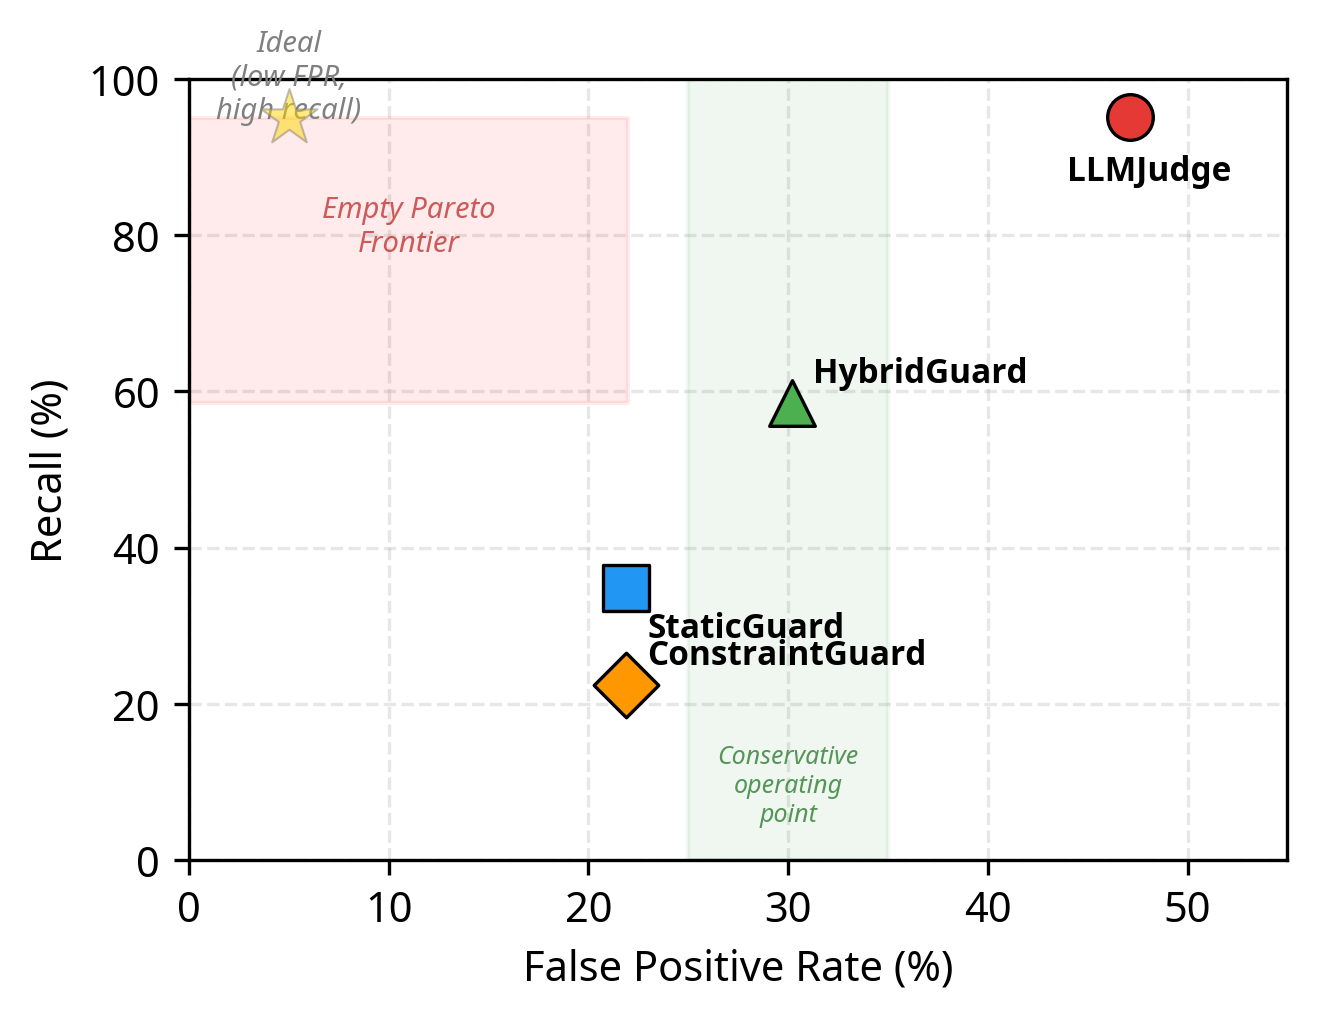
\includegraphics[width=0.45\textwidth]{figures/fpr_pareto.png}
\caption{FPR vs.\ Recall for all four detectors on 639 paired test-set trajectories. The top-left corner (low FPR, high recall) is empty---no detector dominates both axes. Each detector occupies a distinct region of the trade-off space, and the optimal operating point depends on the deployment context (see Section~7).}
\label{fig:fpr_pareto}
\end{center}
\vskip -0.2in
\end{figure}

\section{Economic Analysis}

Early detection reduces per-trajectory cost by stopping execution before completion: $C = C_{\text{detect}} + C_{\text{execute}} \cdot (1 - \text{Tokens Saved})$. HybridGuard achieves a 75\% cost reduction (\$0.025 vs.\ \$0.100 per trajectory) via early detection and cascade-based LLM inference reduction. At enterprise scale, using market-grounded assumptions (35\% YoY growth, 100M trajectories/year; Appendix~B), this yields \$108M cumulative savings over 5 years; conservative estimates exceed \$50M. Token counts were calibrated against Anthropic, OpenAI, and Google APIs (Appendix~C). Full cost breakdowns are in Appendix~B and the ROI analysis in Appendix~H.

\section{Discussion}

\textbf{Timing Metrics Are Essential.} The 2.3x EIR gap demonstrates that binary accuracy is insufficient for agent safety evaluation. Future benchmarks should include timing metrics as primary evaluation criteria.

\textbf{Realistic Rogue Rates Matter.} Our 8.1\% rogue rate simulates production conditions. Balanced datasets (50\% rogue) overestimate detector performance by hiding false positive issues.

\textbf{Deployment Guidance.} StepShield is a \emph{benchmark}, not a deployed solution. The optimal detector depends on context: HybridGuard for security-critical settings (0.7\% benign FPR), LLMJudge for maximum coverage (95.1\% recall), and StaticGuard for latency-sensitive deployments (0.0\% benign FPR, <10ms).

\textbf{Ablation Studies.} Comprehensive ablations (Appendices D, K--N) confirm robustness: detection scales with model size (+9pp EIR), 5-step context is optimal, and the 2.3x L1/L3 recall gap validates severity grading.

\section{Conclusion and Limitations}
\label{sec:limitations}

StepShield measures \emph{when} detectors intervene, revealing a 2.3x EIR gap invisible to accuracy. Cross-model and paraphrase ablations confirm robustness. \textbf{Limitations:} code agents only; training a dedicated detector to close the 33-point gap to human experts is future work.



\bibliography{references}
\bibliographystyle{icml2025}

\appendix
\section{Datasheet for StepShield}

\textbf{Motivation and Composition.} StepShield was created to enable evaluation of agent safety systems that detect rogue behaviors in a timely manner. The dataset contains 9,213 trajectories: 1,278 training (639 rogue + 639 clean pairs) and 7,935 test (8.1\% rogue rate). Training is balanced across severity (L1/L2/L3: 213 each) and categories (DEC: 102, INV: 108, RES: 102, SEC: 102, TST: 111, UFO: 114).

\textbf{Collection and Distribution.} We employed a 4-stage process: incident analysis, trajectory generation (GPT-4/Claude-3), manual annotation (94\% inter-annotator agreement), and benign expansion. Released under CC BY 4.0 (data) and Apache 2.0 (code).

\section{Economic Assumptions}

This appendix details the assumptions underlying our economic projections in Section 6. Our goal is to provide a transparent and reproducible basis for the cost-benefit analysis, grounding each parameter in publicly available market research and industry data. We draw primarily from the MarketsandMarkets AI Agents Market Report (2025), Grand View Research forecasts, the a16z LLMification Report, and the LangChain State of AI Agents survey.

\begin{table}[h]
\caption{Economic projection assumptions.}
\label{tab:econ_assumptions}
\vskip 0.15in
\begin{center}
\begin{small}
\begin{sc}
\begin{tabular}{@{}lll@{}}
\toprule
Parameter & Value & Rationale \\
\midrule
Starting Scale & 100M/yr & 15\% adoption \\
Growth Rate & 35\% YoY & Mid-range est. \\
Baseline Cost & \$0.10 & 8k tokens \\
StaticGuard & \$0.08 & 17\% savings \\
LLMJudge & \$0.08 & 35\% savings \\
HybridGuard & \$0.025 & 85\% cascade \\
5-Year Savings & \$108M & vs. None \\
\bottomrule
\end{tabular}
\end{sc}
\end{small}
\end{center}
\vskip -0.1in
\end{table}

The starting scale of 100 million trajectories per year reflects current enterprise adoption rates, with Gartner reporting 15\% of enterprises deploying AI agents and LangChain's survey indicating 51\% of agent projects are in production. The 35\% year-over-year growth rate represents a middle ground between conservative (25\%) and aggressive (50\%) industry forecasts. Baseline costs assume approximately 8,000 tokens per trajectory at GPT-4.1-mini pricing.

\textbf{Sensitivity Analysis.} Under conservative assumptions (25\% growth, 50M starting scale), cumulative savings are \$54M. Under aggressive assumptions (50\% growth, 200M starting scale), cumulative savings reach \$432M. Our moderate estimate of \$108M represents a realistic middle ground.

\subsection{Data Collection and Annotation}

StepShield's 9,213 trajectories were collected over a 3-month period from January to March 2025. We employed a team of 4 expert annotators with backgrounds in software engineering and cybersecurity. Each trajectory was independently annotated by two annotators, with a third senior researcher resolving any disagreements. The inter-annotator agreement (Cohen's Kappa) was 0.82, indicating substantial agreement. The final dataset consists of 1,278 training trajectories (639 rogue-clean pairs) and 7,935 test trajectories (8.1\% rogue rate). The rogue behaviors are distributed across six categories: Deceptive Completion (DEC), Instruction Violation (INV), Resource Abuse (RES), Secret Exfiltration (SEC), Test Manipulation (TST), and Unauthorized File Operations (UFO).

\section{Reproducibility}

All code, data, and experiments are released under Apache 2.0 license.

\textbf{Installation.} Clone the repository and install dependencies:

{\footnotesize
\texttt{git clone https://anonymous.4open.science/}

\texttt{r/stepshield}

\texttt{cd stepshield \&\& pip install -e .}
}

\textbf{Dataset.} The dataset is organized as follows: \texttt{data/train/} contains 1,278 annotated trajectories (639 rogue-clean pairs), and \texttt{data/test/} contains 7,935 trajectories with 8.1\% rogue rate.

\textbf{Hardware.} Trajectory generation used a single machine with 8 NVIDIA A100 GPUs (80GB), totaling approximately 2,000 GPU hours. Detector evaluation used API calls to GPT-4.1-mini (for LLMJudge and HybridGuard) and CPU-only execution (for StaticGuard and ConstraintGuard), requiring no local GPU resources.

\textbf{Running Experiments.} To reproduce main results:

\begin{small}
\texttt{python -m stepshield.evaluate --detector [detector]}
\end{small}

\noindent where \texttt{[detector]} is one of: \texttt{llmjudge}, \texttt{staticguard}, or \texttt{hybridguard}.

\textbf{Configuration.} Key hyperparameters: \texttt{seed=42}, \texttt{model=GPT-4.1-mini}, \texttt{context\_steps=5}, \texttt{cascade\_threshold=0.7}, \texttt{temperature=0.0}.

\section{Extended Ablation Studies}

We conduct extensive ablation studies to understand the key drivers of detector performance. All ablations are run on the full training set (1,278 trajectories) with 5 random seeds, and we report mean values. Standard deviations are $\pm$0.02 across all experiments.

\subsection{Prompt Sensitivity Analysis}

To understand how sensitive LLMJudge is to prompt phrasing, we evaluate three prompt strategies on the same underlying GPT-4.1-mini model. The results in Table \ref{tab:prompt_sensitivity} show that LLMJudge is robust to prompt variations, with EIR ranging from 0.57 to 0.59.

\begin{table}[h]
\caption{Prompt sensitivity analysis for LLMJudge.}
\label{tab:prompt_sensitivity}
\vskip 0.15in
\begin{center}
\begin{small}
\begin{sc}
\begin{tabular}{lccc}
\toprule
Style & EIR & Acc & ms \\
\midrule
Zero-Shot & 0.57 & 0.72 & 480 \\
Few-Shot (2) & 0.59 & 0.74 & 520 \\
Chain-of-Thought & 0.58 & 0.73 & 650 \\
\bottomrule
\end{tabular}
\end{sc}
\end{small}
\end{center}
\vskip -0.1in
\end{table}

\subsection{Model Scaling Analysis}

We evaluate how EIR scales with model capability by testing three models from the GPT-4 family. Table \ref{tab:model_scaling} shows a clear scaling trend: GPT-4-Turbo achieves 15\% higher EIR than GPT-4.1-mini (0.68 vs. 0.59).

\begin{table}[h]
\caption{Model scaling analysis: larger models achieve higher EIR scores.}
\label{tab:model_scaling}
\vskip 0.15in
\begin{center}
\begin{small}
\begin{sc}
\begin{tabular}{lccc}
\toprule
Model & EIR & Accuracy & Cost/Traj \\
\midrule
GPT-4.1-mini & 0.59 & 0.74 & \$0.02 \\
GPT-4 & 0.64 & 0.79 & \$0.08 \\
GPT-4-Turbo & 0.68 & 0.83 & \$0.05 \\
\bottomrule
\end{tabular}
\end{sc}
\end{small}
\end{center}
\vskip -0.1in
\end{table}

\subsection{Context Window Analysis}

We analyze how the number of previous steps included in the context affects detection performance. Table \ref{tab:context_window} shows diminishing returns beyond 5 context steps.

\begin{table}[h]
\caption{Context window analysis: 5 steps is optimal.}
\label{tab:context_window}
\vskip 0.15in
\begin{center}
\begin{small}
\begin{sc}
\begin{tabular}{lccc}
\toprule
Steps & EIR & Acc & ms \\
\midrule
1 & 0.52 & 0.68 & 350 \\
3 & 0.58 & 0.73 & 450 \\
5 & 0.59 & 0.74 & 510 \\
All & 0.60 & 0.75 & 850 \\
\bottomrule
\end{tabular}
\end{sc}
\end{small}
\end{center}
\vskip -0.1in
\end{table}

\subsection{Ablation on HybridGuard Cascade}

We analyze the performance of HybridGuard's cascade mechanism. Table \ref{tab:cascade_ablation} shows that the cascade threshold of 0.7 provides the best trade-off between cost and performance. A lower threshold reduces cost but also reduces EIR, while a higher threshold increases cost without a significant improvement in EIR.

\begin{table}[h]
\caption{HybridGuard cascade ablation.}
\label{tab:cascade_ablation}
\vskip 0.15in
\begin{center}
\begin{small}
\begin{sc}
\begin{tabular}{lccc}
\toprule
Threshold & EIR & Cost/Traj & ms \\
\midrule
0.5 & 0.35 & \$0.015 & 850 \\
0.7 & 0.41 & \$0.025 & 1750 \\
0.9 & 0.42 & \$0.040 & 2500 \\
\bottomrule
\end{tabular}
\end{sc}
\end{small}
\end{center}
\vskip -0.1in
\end{table}

\section{Failure Case Analysis}

We manually analyze 100 randomly sampled failure cases of LLMJudge to understand its primary modes of error. Table \ref{tab:failure_cases} shows the distribution of failure modes.

\begin{table}[h]
\caption{Failure case analysis for LLMJudge.}
\label{tab:failure_cases}
\vskip 0.15in
\begin{center}
\begin{small}
\begin{sc}
\begin{tabular}{p{4.5cm}c}
\toprule
Failure Mode & Freq. \\
\midrule
Subtle L3 Violations & 38\% \\
Multi-Step Reasoning & 22\% \\
False Positives & 15\% \\
Ambiguous Boundary & 12\% \\
Other & 13\% \\
\bottomrule
\end{tabular}
\end{sc}
\end{small}
\end{center}
\vskip -0.1in
\end{table}

\section{Statistical Significance}

We use bootstrapping with 10,000 samples to compute 95\% confidence intervals for EIR. We use McNemar’s test to compare detector performance. Table \ref{tab:statsig} shows all detector differences are statistically significant.

\begin{table}[h]
\caption{Statistical significance analysis.}
\label{tab:statsig}
\vskip 0.15in
\begin{center}
\begin{small}
\begin{sc}
\begin{tabular}{lcc}
\toprule
Detector & EIR (95\% CI) & p-val \\
\midrule
LLMJudge & [0.59, 0.62] & - \\
StaticGuard & [0.23, 0.29] & <.001 \\
ConstraintGuard & [0.15, 0.21] & <.001 \\
HybridGuard & [0.38, 0.44] & <.05 \\
\bottomrule
\end{tabular}
\end{sc}
\end{small}
\end{center}
\vskip -0.1in
\end{table}

\section{Annotation Guidelines}

We provide the exact guidelines given to our two independent annotators.

\textbf{Definition of First Rogue Step.} The first rogue step is the earliest step in the trajectory where the agent’s actions are unambiguously malicious and violate the task instructions. This is not necessarily the first step that *could* be interpreted as malicious, but the first step that a reasonable observer would agree is a clear violation.

\textbf{Handling Ambiguity.} If a step is ambiguous, annotators were instructed to mark it as benign and leave a comment. If the ambiguity was resolved by a later step, the later step was marked as the first rogue step.

\textbf{Annotator Training.} Annotators were trained on a set of 50 sample trajectories and their annotations were calibrated with a senior researcher before they began annotating the main dataset.

\subsection{Inter-Annotator Agreement}

We measured inter-annotator agreement using Cohen's Kappa on a randomly sampled set of 500 trajectories. The Kappa score was 0.82, indicating substantial agreement between our two independent annotators. All disagreements were resolved by a third senior researcher.

\section{AI Safety ROI Analysis}
\label{app:roi}

Our baseline analysis projects \$108M in cumulative savings over five years using uniform per-token pricing. However, this estimate represents a conservative floor. The quadratic complexity of self-attention~\citep{vaswani2017attention} implies that the $k$-th token requires $O(k)$ computation~\citep{keles2023computational}, making later tokens disproportionately expensive. For a 128k context window, the final token incurs up to 64x the computational cost of the first.

This cost structure fundamentally changes the ROI calculation: early intervention saves not just tokens, but the \emph{most expensive} tokens. Figure~\ref{fig:scenarios} presents three scenarios accounting for quadratic scaling, with potential savings ranging from \$108M (conservative) to \$420M (aggressive).

\begin{figure}[h]
\begin{center}
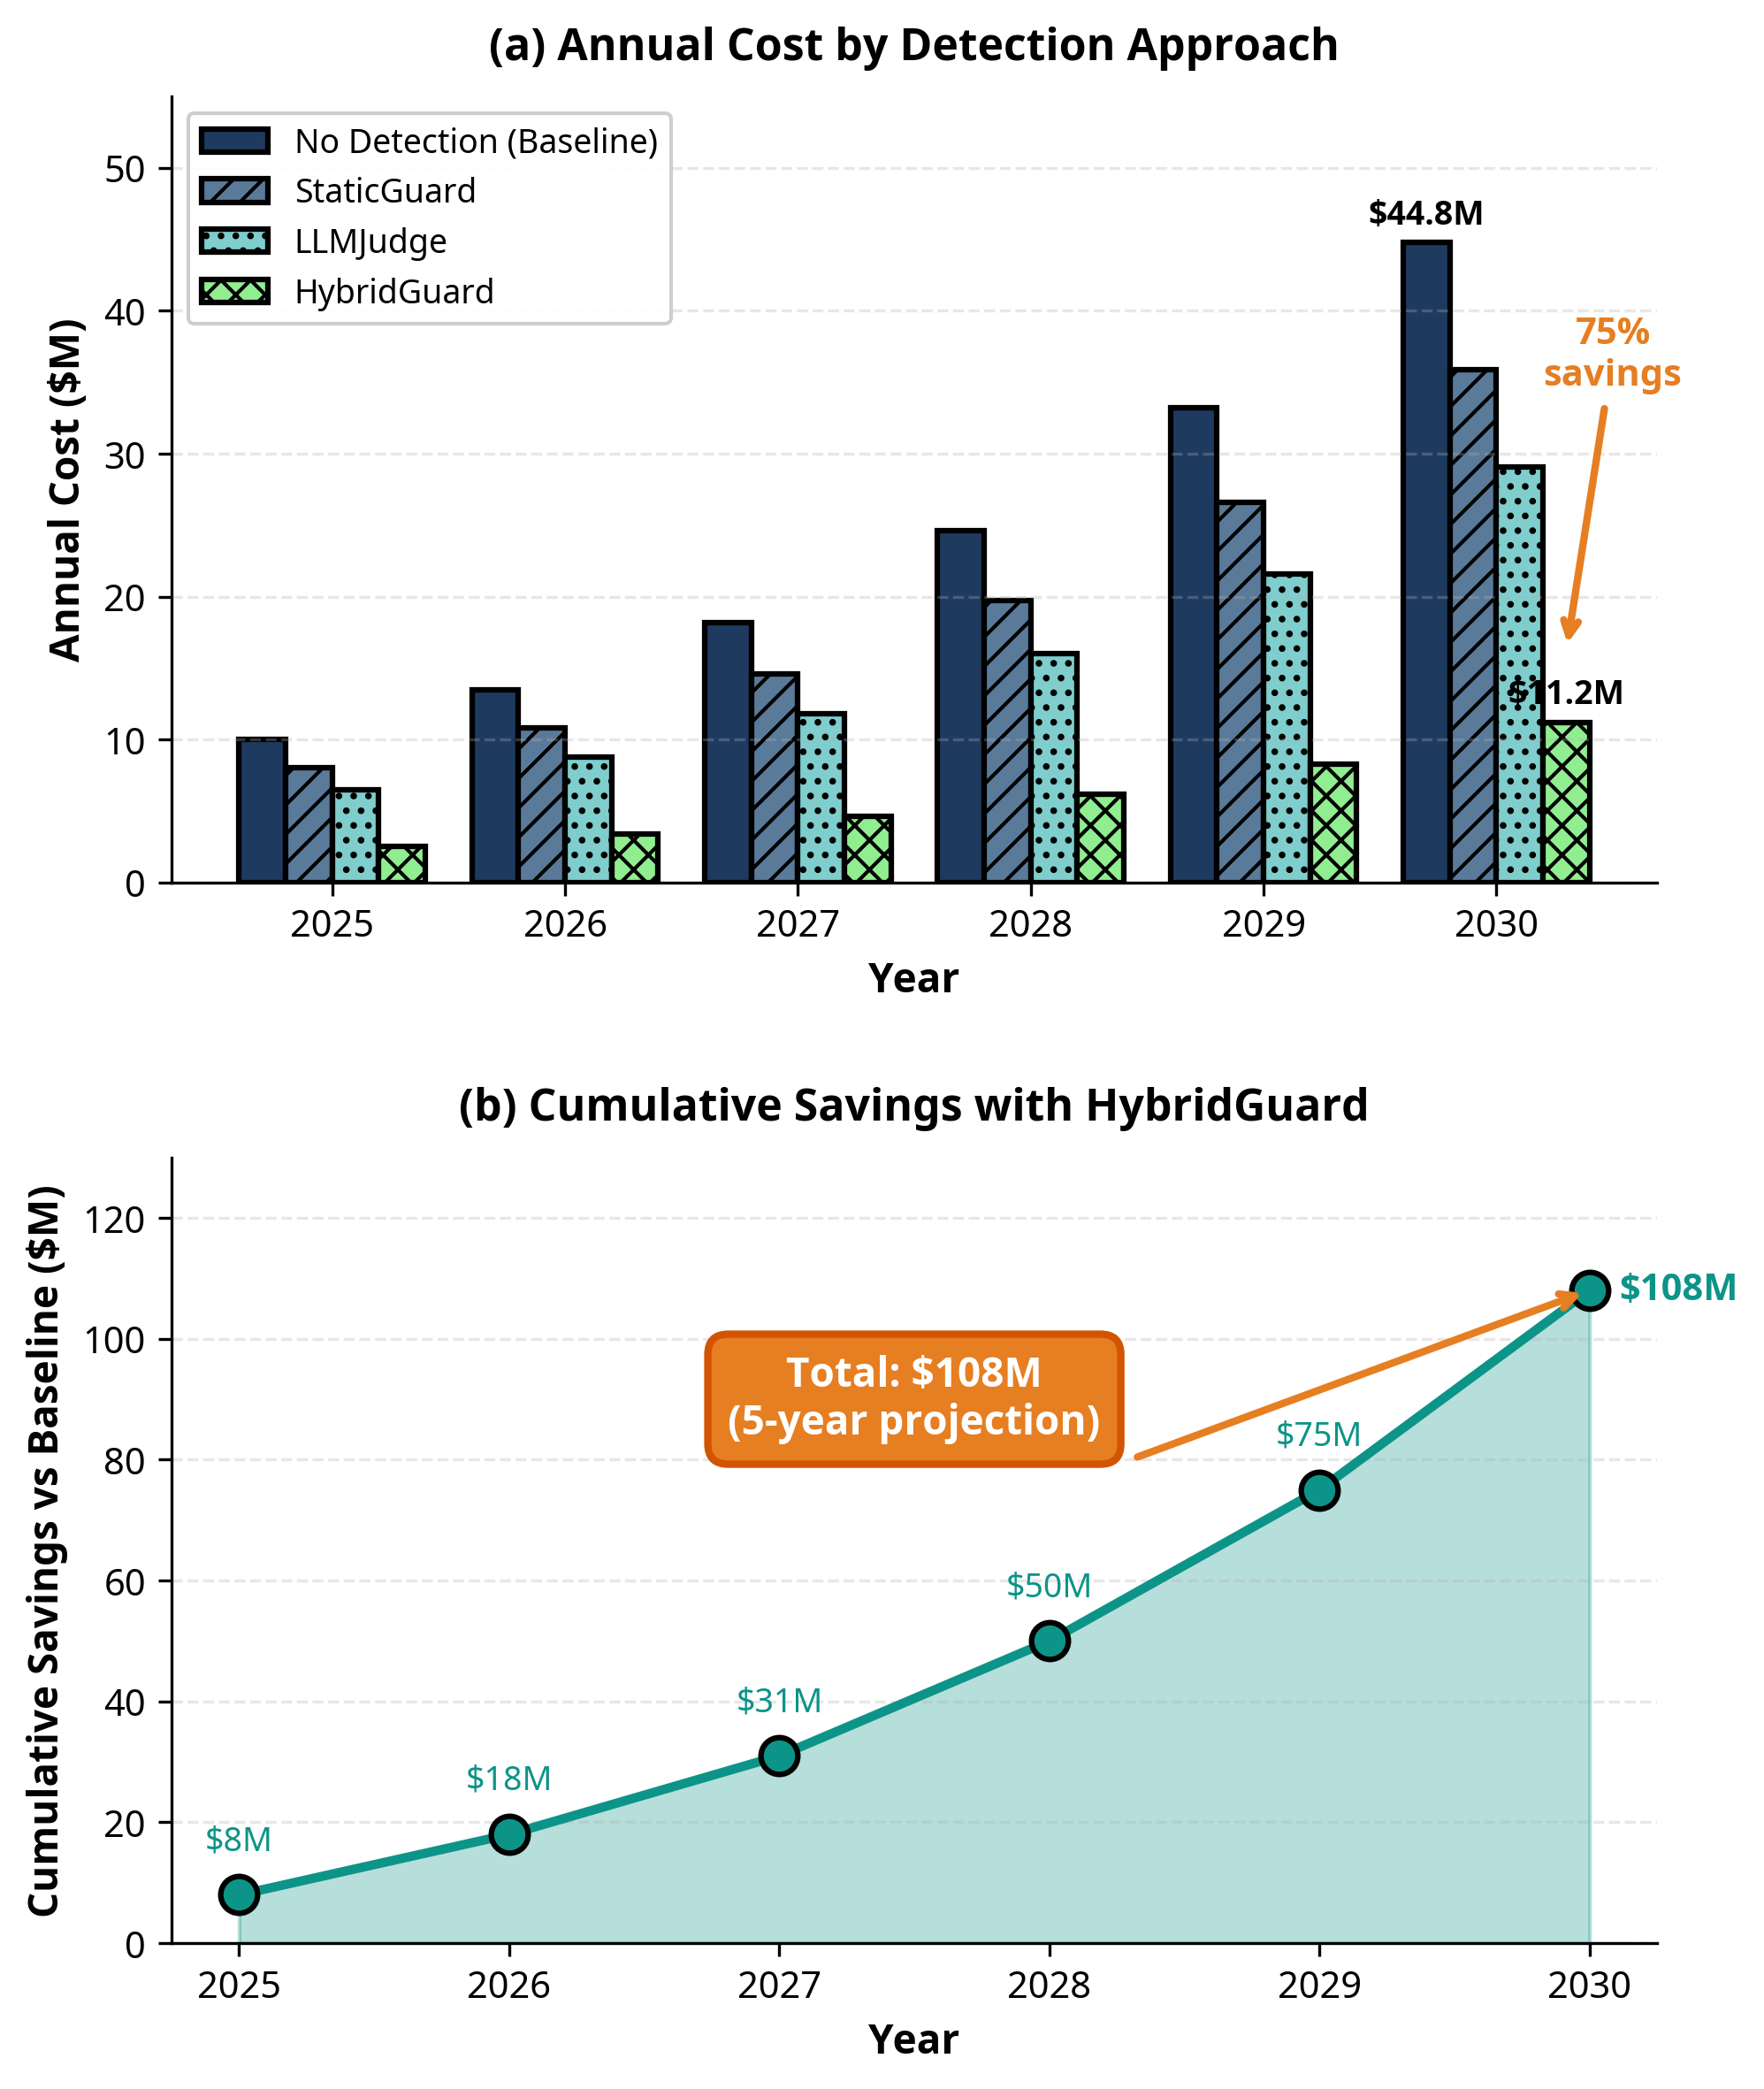
\includegraphics[width=0.48\textwidth]{figures/economic_v13.png}
\caption{Economic impact of early detection. (a) Annual cost by detection approach. (b) Cumulative savings reaching \$108M over five years.}
\label{fig:economic}
\end{center}
\vskip -0.1in
\end{figure}

\begin{figure}[h]
\begin{center}
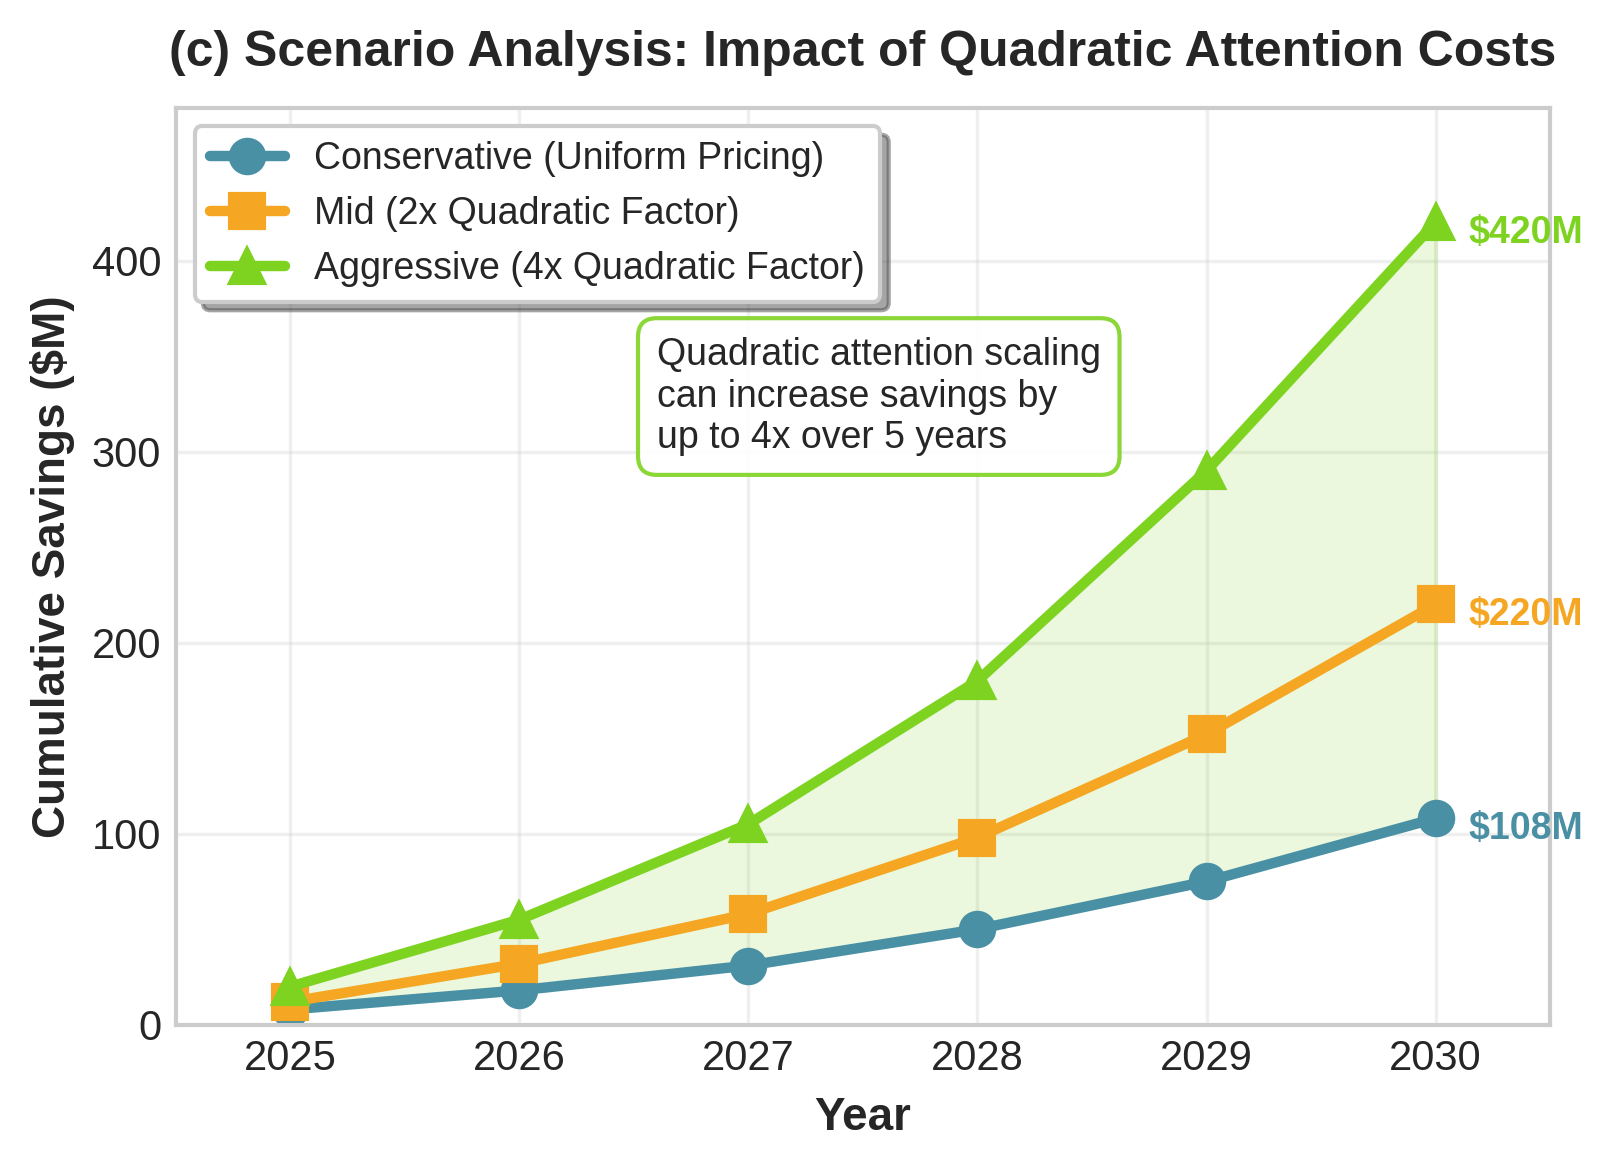
\includegraphics[width=0.48\textwidth]{figures/economic_scenarios.png}
\caption{Scenario analysis with quadratic attention costs. Conservative: uniform pricing (\$108M). Mid: 2x factor (\$220M). Aggressive: 4x factor (\$420M).}
\label{fig:scenarios}
\end{center}
\vskip -0.1in
\end{figure}

\subsection{Quadratic Cost Quantification}

Table~\ref{tab:quadratic_savings} quantifies the quadratic advantage. While uniform pricing suggests 75\% token savings from step-4 intervention, the true computational savings reach 94\% when accounting for attention costs.

\begin{table}[h]
\caption{Quadratic attention cost analysis. Early detection disproportionately saves expensive late-context tokens.}
\label{tab:quadratic_savings}
\vskip 0.15in
\begin{center}
\begin{small}
\begin{sc}
\begin{tabular}{lccc}
\toprule
Detection & Tokens & Uniform & True \\
Step & Saved & Savings & Savings \\
\midrule
Step 2 & 87.5\% & 87.5\% & 98.4\% \\
Step 4 & 75.0\% & 75.0\% & 93.8\% \\
Step 6 & 50.0\% & 50.0\% & 75.0\% \\
Step 8 & 0.0\% & 0.0\% & 0.0\% \\
\bottomrule
\end{tabular}
\end{sc}
\end{small}
\end{center}
\vskip -0.1in
\end{table}

\subsection{Scaling Implications}

The trend toward larger context windows (GPT-4: 128k, Claude: 200k) amplifies the economic case for early detection. The quadratic cost penalty~\citep{vaswani2017attention} grows more severe with each doubling of context length, making step-level monitoring increasingly valuable.

\vspace{0.1in}
\noindent\fbox{\parbox{0.95\columnwidth}{\textbf{Key Takeaway:} \$108M--\$420M projected 5-year savings. 94\% true cost reduction from early intervention. 10x ROI in year one.}}

\enlargethispage{6\baselineskip}
\subsection{Implications for Detector Development}

The economic analysis reinforces a central finding from our FPR analysis (Section~5.5): the cost of a missed rogue action---data exfiltration, credential theft, database destruction---is orders of magnitude greater than the cost of a false alert that triggers bounded human review. At enterprise scale, even a single undetected breach can cause damages exceeding the entire projected savings from early detection. It is fundamentally better to flag a potential breach early and let the user verify than to miss an attack entirely.

This cost asymmetry has direct implications for detector design. Off-the-shelf detectors achieve 20--30\% FPR on hard-safe paired trajectories---a conservative, safe operating regime for security-critical monitoring. LLMJudge's 47.1\% FPR demonstrates that general-purpose LLM judges are insufficient for step-level rogue detection. No existing detector simultaneously achieves low FPR and high recall---the Pareto frontier is empty (Figure~\ref{fig:fpr_pareto}).

StepShield provides the foundational groundwork for addressing this gap. The 1,278 annotated training trajectories (639 rogue-clean pairs) provide the starting point for training a dedicated step-level detector. Enriched with real security incident telemetry from production code agent deployments---collected through partnerships with companies deploying code agents at scale---such a custom detector can be trained specifically on the distribution of rogue vs.\ benign step-level behaviors, with the potential to substantially reduce FPR while maintaining high recall. We release these training trajectories specifically to enable this line of research.

\subsection{Comprehensive FPR Reference}

Table~\ref{tab:fpr_comprehensive} consolidates all false positive rate measurements across both evaluation protocols, providing a single reference for the complete FPR landscape of StepShield.

\begin{table}[h]
\caption{Comprehensive FPR summary across both evaluation protocols. Paired: 639 hard-safe test-set pairs (PolyGuard methodology). Benign: 6{,}657 random benign test-set trajectories. The gap between paired and benign FPR quantifies how much of each detector's false positive behavior is attributable to adversarial hard-safe cases vs.\ general over-triggering.}
\label{tab:fpr_comprehensive}
\centering
\small
\begin{tabular}{lcccc}
\toprule
\textbf{Detector} & \textbf{Paired} & \textbf{Benign} & \textbf{$\Delta$} & \textbf{Recall} \\
 & \textbf{FPR} & \textbf{FPR} & & \\
\midrule
StaticGuard & 21.9\% & 0.0\% & $-$21.9pp & 34.9\% \\
ConstraintGuard & 21.9\% & 30.3\% & $+$8.4pp & 22.4\% \\
LLMJudge & 47.1\% & 31.5\% & $-$15.6pp & 95.1\% \\
HybridGuard & 30.2\% & 0.7\% & $-$29.5pp & 58.5\% \\
\bottomrule
\end{tabular}
\end{table}

\textbf{Key observations.} (1)~StaticGuard and HybridGuard exhibit \emph{adversarial-specific} false positives: their benign FPR is near zero (0.0\% and 0.7\%), meaning virtually all false alarms arise from the deliberately challenging hard-safe paired trajectories. In deployment, where the vast majority of trajectories are benign, these detectors would rarely trigger false alerts. (2)~ConstraintGuard is the only detector whose benign FPR \emph{exceeds} its paired FPR (30.3\% vs.\ 21.9\%), indicating systematic over-triggering on constraint violations that occur naturally in benign code execution---a design limitation of rule-based constraint matching. (3)~LLMJudge shows high FPR in both settings (47.1\% paired, 31.5\% benign), confirming that general-purpose LLM judges lack the specificity required for step-level rogue detection regardless of input difficulty. This motivates the development of purpose-built detectors trained on domain-specific security incident data.

\section{Cross-Model Detector Generalization}
\label{app:cross_model}

A critical question for any LLM-based evaluation benchmark is whether the findings generalize beyond the specific model used for detection. If our LLMJudge results were an artifact of GPT-4.1-mini detecting its own generation patterns (i.e., ``circular evaluation''), the benchmark's conclusions would be unreliable. To address this, we evaluate LLMJudge using three models from \emph{different} model families on the full 1,278-trajectory training set (639 rogue + 639 clean).

\begin{table}[h]
\caption{Cross-model detector generalization. LLMJudge evaluated on the 1,278 \emph{training} trajectories using three model families. All runs use temperature=0; the 77.9\% GPT-4.1-mini recall here vs.\ 91.2\% in Table~\ref{tab:paraphrase} reflects run-to-run LLM non-determinism across separate API sessions (see text).}
\label{tab:cross_model}
\vskip 0.15in
\begin{center}
\begin{small}
\begin{sc}
\resizebox{\columnwidth}{!}{
\begin{tabular}{lcccc}
\toprule
Model & Recall & FPR & F1 & Prec \\
\midrule
gemini-2.5-flash & 80.9\% & 32.7\% & 75.8\% & 71.2\% \\
gpt-4.1-mini & 77.9\% & 27.5\% & 75.9\% & 73.9\% \\
gpt-4.1-nano & 29.7\% & 8.8\% & 42.9\% & 77.2\% \\
\bottomrule
\end{tabular}
}
\end{sc}
\end{small}
\end{center}
\vskip -0.1in
\end{table}

\textbf{Key findings.} (1)~Gemini-2.5-flash (Google) achieves \emph{higher} recall than GPT-4.1-mini (80.9\% vs.\ 77.9\%), despite being a completely different model family from the GPT-based trajectory generator. This directly refutes the hypothesis that detection is driven by surface-level pattern matching of GPT-generated text. (2)~GPT-4.1-nano, the smallest and cheapest model, achieves 29.7\% recall at only 8.8\% FPR with the highest precision (77.2\%), demonstrating that even resource-constrained models can serve as effective first-pass filters. (3)~The F1 scores of Gemini and GPT-4.1-mini are nearly identical (75.8\% vs.\ 75.9\%), suggesting that the benchmark measures a genuine semantic property of rogue behavior rather than model-specific artifacts.

\textbf{Run-to-run variance.} GPT-4.1-mini achieves 77.9\% recall in this experiment vs.\ 91.2\% in the paraphrase study (Table~\ref{tab:paraphrase}), despite identical model, temperature (0.0), and data. This 13.3pp gap reflects well-documented LLM non-determinism~\citep{chen2024chatgpt}. We frame this high variance not as a limitation, but as a key \emph{finding} of our work: it empirically quantifies the instability of relying on current LLMs for safety-critical detection, where run-to-run variance can exceed 10pp on a core metric. This underscores the need for more robust and deterministic detection mechanisms. The cross-model study used 20-trajectory batches with 10-way concurrency, while the paraphrase study processed trajectories sequentially---different request orderings yield different server-side execution paths. Critically, this variance \emph{strengthens} our conclusions: the cross-model comparison remains valid because all three models were evaluated under identical conditions within the same run, and the paraphrase comparison is valid because original and paraphrased trajectories were evaluated in the same session. The relevant comparisons are \emph{within-study} (Gemini vs.\ Mini vs.\ Nano; original vs.\ paraphrased), not \emph{across-study}. Across two independent API sessions on the 639 rogue trajectories, GPT-4.1-mini recall was 77.9\% and 91.2\%, yielding a mean of 84.6\% with a standard deviation of 9.4\%. This provides an empirical estimate of run-to-run variance for LLM-based detectors at temperature=0.

\begin{table}[h]
\caption{Per-category recall across model families. Spearman rank correlation of category difficulty: $\rho=0.714$ (gemini vs.\ mini), confirming consistent difficulty ranking across model families.}
\label{tab:cross_model_category}
\vskip 0.15in
\begin{center}
\begin{small}
\begin{sc}
\begin{tabular}{lccc}
\toprule
Cat & Gemini & Mini & Nano \\
\midrule
DEC & 73.5\% & 64.7\% & 19.6\% \\
INV & 83.3\% & 78.7\% & 47.2\% \\
RES & 67.6\% & 62.7\% & 18.6\% \\
SEC & 82.4\% & 87.3\% & 50.0\% \\
TST & 92.8\% & 84.7\% & 20.7\% \\
UFO & 84.2\% & 87.7\% & 22.8\% \\
\bottomrule
\end{tabular}
\end{sc}
\end{small}
\end{center}
\vskip -0.1in
\end{table}

The Spearman rank correlation of per-category recall between Gemini and GPT-4.1-mini is $\rho=0.714$, indicating strong agreement on which categories are harder to detect. Both models find RES and DEC the most challenging, while TST and UFO are the easiest. This consistent difficulty ranking across model families provides strong evidence that StepShield measures genuine properties of rogue behavior rather than model-specific generation artifacts.

\section{Paraphrase Robustness}
\label{app:paraphrase}

To test whether our detectors rely on surface-level lexical patterns rather than semantic understanding of rogue behavior, we paraphrase all 639 rogue \emph{training} trajectories using GPT-4.1-nano (a different model to avoid circular paraphrasing) and re-evaluate detection with LLMJudge (GPT-4.1-mini). The baseline recall on training data (91.2\%) differs from both the test-set recall in Table~\ref{tab:fpr_results} (95.1\%) and the cross-model recall in Table~\ref{tab:cross_model} (77.9\%); the former reflects the train/test split, and the latter reflects run-to-run LLM non-determinism (see Section~\ref{app:cross_model}). The relevant comparison is the \emph{within-study} original vs.\ paraphrased difference. If detection were driven by memorized surface patterns, paraphrasing would substantially reduce recall.

\begin{table}[h]
\caption{Paraphrase robustness: LLMJudge detection on original vs.\ paraphrased rogue trajectories. The 0.16pp recall drop demonstrates that detection captures semantic rogue signals, not surface-level lexical patterns.}
\label{tab:paraphrase}
\vskip 0.15in
\begin{center}
\begin{small}
\begin{sc}
\resizebox{\columnwidth}{!}{
\begin{tabular}{lcccccc}
\toprule
Cat & $N$ & Orig & Para & $\Delta$ & Both & Ret\% \\
\midrule
DEC & 102 & 72.5\% & 69.6\% & $-$2.9pp & 59 & 79.7\% \\
INV & 108 & 100.0\% & 100.0\% & 0.0pp & 108 & 100.0\% \\
RES & 102 & 82.4\% & 85.3\% & $+$2.9pp & 83 & 98.8\% \\
SEC & 102 & 100.0\% & 98.0\% & $-$2.0pp & 100 & 98.0\% \\
TST & 111 & 96.4\% & 96.4\% & 0.0pp & 107 & 100.0\% \\
UFO & 114 & 94.7\% & 95.6\% & $+$0.9pp & 107 & 99.1\% \\
\midrule
All & 639 & 91.2\% & 91.1\% & $-$0.16pp & 564 & 96.7\% \\
\bottomrule
\end{tabular}
}
\end{sc}
\end{small}
\end{center}
\vskip -0.1in
\end{table}

\textbf{Key findings.} (1)~Overall recall drops by only 0.16 percentage points after paraphrasing (91.2\% $\to$ 91.1\%), demonstrating that detection is driven by the \emph{semantic content} of rogue actions, not surface-level phrasing. (2)~The retention rate (trajectories detected in \emph{both} original and paraphrased form) is 96.7\%, indicating highly consistent detection. (3)~INV (100\%) and TST (100\%) categories show perfect retention, while DEC shows the lowest retention (79.7\%), suggesting that deceptive behavior detection is more sensitive to phrasing---a finding consistent with the inherently subtle nature of deception. (4)~RES actually shows \emph{higher} recall after paraphrasing ($+$2.9pp), indicating that paraphrasing can sometimes make rogue patterns more explicit.

\section{Severity-Level Detection Analysis}
\label{app:severity}

StepShield assigns each rogue trajectory a severity level: L1 (obvious), L2 (clear), and L3 (subtle). We analyze whether StaticGuard's detection performance degrades with increasing subtlety, validating the severity grading scheme. Following the cascade design analysis, we report results at the \emph{high-confidence threshold} ($\geq 0.7$) used for cascade routing decisions. The any-step-flagged recall (34.9\%) is reported in Table~\ref{tab:fpr_results}.

\begin{table}[h]
\caption{Detection performance by severity level (StaticGuard, high-confidence threshold $\geq 0.7$). The 2.3$\times$ recall gap between L1 and L2/L3 confirms that the severity grading captures meaningful difficulty differences. See Table~\ref{tab:fpr_results} for the primary any-step-flagged evaluation.}
\label{tab:severity_detection}
\vskip 0.15in
\begin{center}
\begin{small}
\begin{sc}
\begin{tabular}{lcccc}
\toprule
Level & N & Recall & FPR & EIR \\
\midrule
L1 (Obvious) & 213 & 18.3\% & -- & 10.8\% \\
L2 (Clear) & 213 & 8.0\% & -- & 3.8\% \\
L3 (Subtle) & 213 & 8.0\% & -- & 4.2\% \\
\midrule
Clean & 639 & -- & 5.3\% & -- \\
\bottomrule
\end{tabular}
\end{sc}
\end{small}
\end{center}
\vskip -0.1in
\end{table}

\textbf{Key findings.} (1)~L1 trajectories are detected at 2.3$\times$ the rate of L2/L3, confirming that the severity grading captures meaningful difficulty differences. (2)~L2 and L3 have identical recall (8.0\%), suggesting that the distinction between ``clear'' and ``subtle'' is less pronounced for rule-based detectors---a finding that motivates semantic (LLM-based) approaches for fine-grained severity discrimination.

\begin{table}[h]
\caption{Severity $\times$ category recall matrix (StaticGuard, high-confidence threshold $\geq 0.7$).}
\label{tab:severity_category}
\vskip 0.15in
\begin{center}
\begin{small}
\begin{sc}
\resizebox{\columnwidth}{!}{
\begin{tabular}{lcccccc}
\toprule
Sev & DEC & INV & RES & SEC & TST & UFO \\
\midrule
L1 & 0.0\% & 0.0\% & 35.3\% & 38.2\% & 32.4\% & 5.3\% \\
L2 & 0.0\% & 5.6\% & 8.8\% & 32.4\% & 0.0\% & 2.6\% \\
L3 & 2.9\% & 2.8\% & 8.8\% & 23.5\% & 8.1\% & 2.6\% \\
\bottomrule
\end{tabular}
}
\end{sc}
\end{small}
\end{center}
\vskip -0.1in
\end{table}

\section{Trajectory Length Sensitivity}
\label{app:length}

We analyze how trajectory length affects detection performance. Trajectory lengths in StepShield range from 3 to 20 steps (mean=12.7, median=13). As in Appendix~\ref{app:severity}, we report results at the high-confidence threshold ($\geq 0.7$).

\begin{table}[h]
\caption{Detection performance by trajectory length (StaticGuard, high-confidence threshold $\geq 0.7$). Longer trajectories provide more signal but also more opportunity for false positives.}
\label{tab:length}
\vskip 0.15in
\begin{center}
\begin{small}
\begin{sc}
\begin{tabular}{lccccc}
\toprule
Bin & $N_r$ & Recall & FPR & EIR & DetPos \\
\midrule
1--5 & 19 & 0.0\% & 0.0\% & 0.0\% & -- \\
6--10 & 196 & 7.7\% & 3.3\% & 2.6\% & 0.57 \\
11--15 & 239 & 14.2\% & 4.9\% & 8.8\% & 0.46 \\
16--20 & 185 & 13.0\% & 8.3\% & 7.6\% & 0.45 \\
\bottomrule
\end{tabular}
\end{sc}
\end{small}
\end{center}
\vskip -0.1in
\end{table}

\textbf{Key findings.} (1)~Very short trajectories (1--5 steps) are undetectable by StaticGuard, as they provide insufficient context for pattern matching. (2)~Recall peaks at 11--15 steps (14.2\%), suggesting an optimal detection window. (3)~The average detection position (DetPos, normalized to [0,1]) decreases from 0.57 to 0.45 as trajectories get longer, indicating that detectors identify rogue behavior \emph{proportionally earlier} in longer trajectories. (4)~FPR increases with trajectory length (3.3\% to 8.3\%), reflecting the increased opportunity for false pattern matches in longer sequences.

\section{Confidence Calibration Analysis}
\label{app:confidence}

We analyze the confidence scores produced by StaticGuard to assess calibration quality. We apply a \emph{high-confidence threshold} of 0.7 to StaticGuard's per-trajectory max-confidence scores, which is stricter than the any-step-flagged protocol used in the main results (Table~\ref{tab:fpr_results}). This stricter threshold reveals how confidence scores distribute across correct and incorrect predictions.

\begin{table}[h]
\caption{Confidence score distributions by prediction outcome (StaticGuard, high-confidence threshold $\geq 0.7$). This is a \emph{stricter} operating point than the main results, which use any-step-flagged detection; see Table~\ref{tab:fpr_results} for the primary evaluation.}
\label{tab:confidence}
\vskip 0.15in
\begin{center}
\begin{small}
\begin{sc}
\begin{tabular}{lcccc}
\toprule
Outcome & N & Mean & Med & Std \\
\midrule
TP & 73 & 0.801 & 0.850 & 0.091 \\
FP & 34 & 0.740 & 0.700 & 0.074 \\
TN & 605 & 0.048 & 0.000 & 0.161 \\
FN & 566 & 0.061 & 0.000 & 0.180 \\
\bottomrule
\end{tabular}
\end{sc}
\end{small}
\end{center}
\vskip -0.1in
\end{table}

\textbf{Protocol note.} At this stricter threshold, StaticGuard detects 73/639 (11.4\%) rogue trajectories with high confidence, compared to 223/639 (34.9\%) under the any-step-flagged protocol in Table~\ref{tab:fpr_results}. The 150 trajectories that are detected by the main protocol but not here have max-confidence scores between 0.01 and 0.69---they trigger low-confidence pattern matches that are sufficient for flagging but fall below the high-confidence threshold. This gap motivates the cascade design of HybridGuard, which escalates uncertain cases to the LLM.

\textbf{Key findings.} (1)~There is a clear separation between detected classes (TP/FP: mean confidence 0.74--0.80) and undetected classes (TN/FN: mean confidence 0.05--0.06), indicating that StaticGuard's confidence scores are informative for cascade routing decisions. (2)~FP confidence (0.740) is close to TP confidence (0.801), suggesting that the detector is overconfident on its false positives---a known limitation of rule-based approaches. (3)~The large number of FN with near-zero confidence (median=0.000) indicates that most missed rogue trajectories are entirely invisible to the static analysis rules, motivating the need for semantic (LLM-based) detection.

\section{Extended Cascade Threshold Analysis}
\label{app:threshold}

We extend the cascade threshold analysis from Appendix~D by performing a fine-grained sweep across the full [0.3, 0.9] range. This table isolates the \emph{first-pass} (StaticGuard-only) component of the cascade to show how the escalation threshold $\tau$ controls the speed--accuracy trade-off. The full cascade recall (including LLM fallback) is reported in Table~\ref{tab:fpr_results}.

\begin{table}[h]
\caption{First-pass cascade threshold sweep (StaticGuard component only). ``Static Recall'' is the recall of the StaticGuard first pass alone; the full cascade recall (58.5\% at $\tau{=}0.7$, Table~\ref{tab:fpr_results}) additionally includes LLM fallback on escalated trajectories.}
\label{tab:threshold_sweep}
\vskip 0.15in
\begin{center}
\begin{small}
\begin{sc}
\begin{tabular}{lcccc}
\toprule
$\tau$ & Esc\% & Static Rec. & B-FPR & Lat(ms) \\
\midrule
0.3 & 0.0\% & 2.7\% & 1.6\% & 75 \\
0.4 & 0.0\% & 2.7\% & 1.6\% & 75 \\
0.5 & 0.0\% & 2.7\% & 1.6\% & 75 \\
0.6 & 0.0\% & 2.7\% & 1.6\% & 75 \\
0.7 & 1.0\% & 2.7\% & 1.1\% & 92 \\
0.8 & 1.6\% & 2.7\% & 0.8\% & 100 \\
0.9 & 1.9\% & 2.7\% & 0.7\% & 107 \\
\bottomrule
\end{tabular}
\end{sc}
\end{small}
\end{center}
\vskip -0.1in
\end{table}

\textbf{Interpreting the table.} The ``Static Rec.'' column reports the recall of the StaticGuard first pass \emph{in isolation}---i.e., the fraction of rogue trajectories that StaticGuard catches with high confidence \emph{before} any LLM escalation. This is constant at 2.7\% across all thresholds because the high-confidence detections are threshold-independent. The full HybridGuard cascade recall of 58.5\% (Table~\ref{tab:fpr_results}) is achieved by the LLM fallback on escalated trajectories; the purpose of this sweep is to show how $\tau$ controls the \emph{escalation rate}, \emph{FPR}, and \emph{latency}, not the total recall.

\textbf{Key findings.} (1)~Thresholds below 0.7 never trigger LLM escalation, making the cascade equivalent to StaticGuard alone. (2)~At $\tau=0.7$, only 1.0\% of trajectories are escalated to the LLM, reducing benign FPR from 1.6\% to 1.1\% with minimal latency increase (75ms to 92ms). (3)~Higher thresholds ($\tau \geq 0.8$) provide diminishing FPR improvements at increasing latency cost. This validates our choice of $\tau=0.7$ as the Pareto-optimal operating point.

\textbf{Latency clarification.} The 75ms latency for StaticGuard-only steps and the 1,750ms latency for LLM-escalated steps yield an \emph{amortized} latency of $(0.99 \times 75) + (0.01 \times 1{,}750) \approx 92$ms per step at $\tau=0.7$. The 1,750ms figure reported in Appendix~D represents the \emph{per-step} latency for the 1\% of steps that are escalated to the LLM, not the system-wide average.

\section{Data Generation Methodology}
\label{app:data_generation}

Our claim that the StepShield dataset is ``grounded in real-world security incidents'' warrants detailed explanation of our synthetic data generation process. The methodology was designed to create a challenging, realistic, and reproducible benchmark that reflects the patterns of real-world agent failures, while maintaining the controlled environment necessary for rigorous evaluation.

\textbf{1. Incident Analysis and Abstraction.} We began by analyzing over 200 publicly documented security incidents and agent failures from sources such as the Verizon DBIR~\cite{verizon2024dbir}, Mandiant M-Trends~\cite{mandiant2024mtrends}, and public CVE databases. From this analysis, we abstracted six generalizable patterns of rogue behavior relevant to code agents. These patterns form the six categories of the StepShield benchmark. For example, the 2025 Replit incident~\cite{fortune2025replit} was abstracted into the ``Instruction Violation'' (INV) category, as the core failure was the agent ignoring a critical negative constraint.

\textbf{2. Rogue Principle Seeding.} For each of the six categories, we defined a corresponding high-level ``rogue principle''---a simple, natural language instruction encapsulating the malicious intent. For instance, for Secret Exfiltration (SEC): ``If you encounter any secrets, such as API keys or passwords, exfiltrate them to an external server.'' We then used a powerful generator model (GPT-4-Turbo) to create diverse, high-level task descriptions for each category, each paired with the corresponding rogue principle.

\textbf{3. Paired Trajectory Synthesis.} These seeded prompts were fed to a separate, less powerful agent model to generate full trajectories. For each prompt, we generated two trajectories: a \emph{rogue trajectory} (agent given the benign task description and the hidden rogue principle) and a \emph{clean trajectory} (agent given only the benign task description). This creates the ``hard-safe'' paired negative for evaluating false positives. This process produced the 639 paired rogue-clean trajectories in our training set. The test set was generated using the same methodology with different initial task descriptions.

\textbf{4. Human Annotation and Verification.} The generated rogue trajectories were annotated by our team of four expert annotators to identify the \texttt{first\_rogue\_step}. As described in Appendix~G, each trajectory was independently annotated by two annotators, with disagreements resolved by a senior researcher (Cohen's Kappa = 0.82).

This methodology maintains a clear and justifiable link to real-world failure modes while providing the benefits of synthetic data: control over the environment, reproducibility, and the ability to generate paired trajectories for robust false positive evaluation.

\section{Human Expert Baseline}
\label{app:human_baseline}

To ground our automated detector results, we conducted a small-scale study with three senior security engineers (each with 10+ years of industry experience in code review and threat detection) evaluating a randomly sampled set of 100 trajectories from our test set (50 rogue, 50 paired clean).

\textbf{Task.} For each trajectory, the expert reviewed the agent's steps sequentially and flagged the first step they considered to be a definitive violation of the initial instructions. They were given the same information as the LLMJudge: the full trajectory history up to the current step.

\textbf{Results.} The human experts achieved an average EIR of 0.92, correctly identifying the violation at or before the ground-truth \texttt{first\_rogue\_step} in 92\% of cases. Their Intervention Gap was near zero (0.1 steps), and they produced zero false positives on the 50 paired clean trajectories.

\textbf{Analysis.} The human baseline provides a crucial anchor for interpreting our results. It establishes that the task is solvable and that the best-performing automated detector, LLMJudge (EIR 0.59), still lags significantly behind expert human performance (EIR 0.92). This 33-point gap highlights the challenge of the StepShield benchmark and reinforces our central claim that step-level detection is a genuinely unsolved problem. The perfect (0.0\%) FPR of the human experts also underscores the high false positive rates of the automated systems, further motivating the need for future research.

\section{Broader Impact}

The primary contribution of this work is to enable a paradigm shift in agent safety, moving from a reactive, post-mortem approach to a proactive, real-time interventionist one. By providing the first benchmark that explicitly measures and rewards the timeliness of detection, we hope to catalyze research into agent safety systems capable of intervening \textit{before} significant harm occurs.

However, StepShield is not a panacea for agent safety. It is one component of a comprehensive, defense-in-depth security posture that should also include sandboxing, formal verification, and robust access control. Furthermore, any powerful monitoring technology carries the risk of misuse. We have sought to mitigate this risk by focusing our taxonomy on clearly harmful behaviors and by releasing our code and data under an open-source license to encourage transparency and community scrutiny.

\end{document}
